\documentclass[journal]{IEEEtran}

\usepackage{amsmath,amssymb,amsfonts}
\usepackage{graphicx}
\usepackage{booktabs}
\usepackage{cite}
\usepackage{url}
\usepackage{array}
\usepackage{multirow}
\usepackage{balance}

\graphicspath{{figures/source_from_dissertation/}{figures/generated/}{figures/tcds_hardening/}}

\newcommand{\E}{\mathcal{E}}
\newcommand{\D}{\mathcal{D}}
\newcommand{\T}{\mathcal{T}}
\newcommand{\C}{\mathcal{C}}
\newcommand{\BA}{\mathrm{BA}}
\newcommand{\AUC}{\mathrm{AUC}}
\newcommand{\R}{\mathbb{R}}
\newcommand{\KL}{\mathrm{KL}}
\newcommand{\Hent}{\mathcal{H}}

\begin{document}

\title{Operational Distinctness in Staged Neuromorphic Architectures: A Layer Ablation Analysis of Clinical EEG}

\author{Andrew A. Lane, K. Wendy Tang, and Brady D. Nelson%
\thanks{This manuscript was prepared from privacy-preserving reporting outputs and the TCDS submission-hardening pipeline (parallelized permutation-FDR inference, $\kappa$-coupling analysis, reservoir-dynamics visualization, and an embodied closed-loop active-inference demonstration). Affective-task significance is reported with subject-respecting permutation tests at $n_{\mathrm{perm}}=200$. Clinical-label sensitivity is reported with Benjamini--Hochberg FDR correction across the 30 diagnosis $\times$ configuration tests; no clinical contrast survived FDR at $\alpha=0.05$, and clinical findings are presented as weak-signal sensitivity rather than biomarker validation.}%
}

\maketitle

\begin{abstract}
Brain-inspired computing for embodied AI requires architectures whose components are grounded in concrete neural mechanisms rather than loose metaphors. We instantiate this requirement in Affective Reservoir-Spike Processing and Inference Network (ARSPI-Net), a staged neuromorphic architecture for clinical affective electroencephalography (EEG) that combines a fixed leaky integrate-and-fire (LIF) spiking reservoir, a binned spike-count (BSC$_6$) neural-coding scheme, electrode-level temporal-phase-locking topology, and a structure--function coupling readout $\kappa = \|C\|_F/\sqrt{p\,q}$. ARSPI-Net produces four operationally distinct feature families: a spike-coded reservoir embedding $E$, dynamical descriptors $D$, graph-topological descriptors $T$, and the coupling block $C$. We evaluate \emph{operational distinctness}---empirical non-equivalence of layers under a fixed evaluation protocol---across 633 subject-condition observations from 211 subjects under subject-grouped cross-validation. With subject-respecting permutation tests ($n_{\mathrm{perm}}=200$), 8 of 10 affective configurations exceed chance at $p \leq 0.005$, including BandPower (49.27\%), $E$ (46.96\%), $E+D$ (49.34\%), and $E+D+T+C$ (49.33\%); $T$ alone and $C$ alone do not. Across 30 Benjamini--Hochberg-adjusted clinical contrasts, no diagnosis reaches FDR significance ($\min p_{\mathrm{BH}} = 0.30$), so clinical layer-profile differences are reported as weak-signal sensitivity, not biomarker validation. Three brain-inspired-mechanism analyses extend the operational-distinctness audit. (i)~A 5{,}000-permutation electrode-shuffle test of $\kappa$ rejects the structure-permuted null in 33.5\% of observations; mean $\kappa = 0.250$ (sd $0.115$). (ii)~A reservoir-dynamics figure surfaces the LIF spike rasters, membrane trajectories, per-class temporal-phase-locking matrices, and BSC$_6$ projection underlying the embedding. (iii)~A simulated embodied closed-loop active-inference agent that attends to ARSPI-Net feature streams discriminates layer utility by per-step expected information gain over a Dirichlet posterior; the full $E+D+T$ stream reduces posterior predictive entropy fastest (final entropy $0.93$ nats) and the topological-only stream slowest ($1.08$ nats), consistent with the offline ablation result. Pairwise centered-kernel alignment values are low-to-moderate (largest $\mathrm{CKA}(E,D)=0.31$), supporting non-equivalence of the layer spaces. Together, these results establish ARSPI-Net layers as operationally distinct measurement views suitable as a multi-stream substrate for embodied AI, while honestly bounding clinical claims to the weak-signal regime supported by FDR-corrected inference.
\end{abstract}

\begin{IEEEkeywords}
EEG, neuromorphic computing, spiking neural networks, liquid state machines, reservoir computing, neural coding, predictive coding, active inference, embodied AI, perception--action loops, structure--function coupling, clinical-label sensitivity, layer ablation, operational distinctness.
\end{IEEEkeywords}

\section{Introduction}
Electroencephalography (EEG) provides millisecond-scale access to neural activity, but scalp recordings are noisy, indirect, subject-dependent observations of latent neural dynamics. Clinical affective EEG is particularly difficult because affective stimulus responses, inter-subject covariance, comorbidity, medication, and nonstationarity coexist in the same measurement. A single endpoint classifier can be useful, but it does not by itself determine which component of a staged architecture carries information, whether later layers add discriminative utility, or whether intermediate representations measure distinct signal properties.

Recent IEEE biomedical and neural-systems papers set a high methodological bar for EEG architectures. Compact EEG convolutional baselines such as EEGNet~\cite{lawhern2018eegnet}, EEG graph neural networks~\cite{klepl2024gnn,klepl2023ad}, and spiking/graph hybrids~\cite{gong2023sglnet} are typically evaluated through cross-subject protocols, ablations, multiple metrics, and architectural diagrams. Biomedical informatics studies similarly report modality-specific comparisons, ablation logic, and cross-subject validation when proposing physiological classifiers~\cite{guo2025mma,chiang2023depression}. These papers highlight a standard that the present study follows: a staged architecture is not adequately justified by a single final accuracy value. Its modules must be evaluated by what they contribute.

This paper studies this problem in Affective Reservoir-Spike Processing and Inference Network (ARSPI-Net), a staged neuromorphic EEG architecture. ARSPI-Net maps each event-related EEG observation into several feature families: a reservoir spike embedding $E$, dynamical descriptors $D$, graph-topological descriptors $T$, and structure-function coupling descriptors $C$. Earlier ARSPI-Net manuscripts addressed different questions: one characterized subject-covariance structure, and another defined a four-level interpretability framework. The present manuscript asks a more architectural question: are the ARSPI-Net layers operationally distinct, or are they redundant feature blocks?

We define operational distinctness as empirical non-equivalence of layers under a fixed evaluation protocol. A layer may be operationally distinct if it differs in predictive sufficiency, incremental utility, clinical-label sensitivity, or representational redundancy. This definition is intentionally measurement-oriented. It does not assert that layers correspond to independent biological mechanisms. It asks whether they behave as different signal-processing views of the same EEG response.

The framing aligns with the IEEE TCDS Special Issue on Brain-Inspired Computing for Embodied AI in two ways. First, ARSPI-Net's mechanism is concrete and not metaphorical: the reservoir is a fixed leaky integrate-and-fire spiking network~\cite{maass2002liquid}, the embedding $E$ is produced by a binned-spike-count neural-coding scheme, and the topological block $T$ rests on temporal-phase-locking connectivity matrices that respect the cortical-network organisation surveyed by Bullmore and Sporns~\cite{bullmore2009complex}. Second, we evaluate the architecture not only as an offline classifier but also as a perception--action substrate for an embodied agent. Specifically, we simulate a closed-loop active-inference agent~\cite{friston2010free,parr2022activeinference} that maintains a Dirichlet posterior over a held-out subject's affective response and chooses, at each step, which ARSPI-Net feature stream (E, D, T, or full E+D+T) to attend to. Different streams correspond to operationally distinct cortical-style sub-systems and yield different per-step expected information gains; this yields a direct embodied-AI test of layer utility that complements the offline ablation.

The contributions are fivefold:
\begin{enumerate}
    \item We formalize a layer-ablation test for staged neuromorphic EEG architectures and ground each block in a concrete neural mechanism (LIF spiking, BSC$_6$ neural coding, tPLV connectivity, structure--function coupling).
    \item We evaluate ARSPI-Net feature families $E$, $D$, $T$, and $C$ under a controlled A0--A9 affective ablation and C1--C6 clinical-label sensitivity matrix with subject-respecting permutation inference and Benjamini--Hochberg FDR correction.
    \item We report feature diagnostics, layer redundancy (CKA), comorbidity-adjusted exploratory models, and a 5{,}000-permutation electrode-shuffle null for the structure--function coupling readout $\kappa$.
    \item We distinguish predictive utility from measurement utility, showing that ARSPI-Net layers are target-dependent rather than a monotonic accuracy stack.
    \item We instantiate ARSPI-Net as the perception substrate of a simulated embodied closed-loop active-inference agent and quantify per-policy expected-information-gain rates, providing an embodied-AI test of layer utility that complements the offline ablation.
\end{enumerate}

\section{Related Work and Novelty Boundary}
\subsection{EEG Classification and Biomedical Evaluation Norms}
EEG classification papers commonly compare new representations against compact neural baselines, spectral features, recurrent models, and graph-based models~\cite{lawhern2018eegnet,craik2019deep,klepl2024gnn}. In TNSRE, Gong \emph{et al.} integrated spike encoding, adaptive graph convolution, and spike-based LSTM units for EEG-based BCI and reported cross-subject evaluation, parameter analysis, and confusion matrices~\cite{gong2023sglnet}. In JBHI, Guo \emph{et al.} proposed a multimodal attention network for EEG/EDA/PPG fatigue detection and reported cross-subject experiments and modality comparisons~\cite{guo2025mma}. These examples motivate the present manuscript's structure: architecture, mathematical definition, controlled ablation, multiple metrics, claim-bounded clinical discussion, and reproducible outputs.

\subsection{Graph and Spiking EEG Models}
Graph neural networks have been used for emotion recognition, motor imagery, and neurological or psychiatric classification from EEG. Klepl \emph{et al.} emphasized that EEG-GNN methods differ substantially in node features, graph construction, graph convolution, pooling, and readout choices~\cite{klepl2024gnn}. Spiking methods add temporal event-based computation and dynamical state variables~\cite{maass2002liquid,gong2023sglnet}. ARSPI-Net differs from end-to-end EEG classifiers by treating the reservoir as a fixed nonlinear measurement operator whose outputs support multiple downstream descriptors.

\subsection{Novelty Boundary Relative to Prior ARSPI-Net Work}
The novelty of this paper is not the mere existence of ARSPI-Net, nor the claim that ARSPI-Net is interpretable. The unique question is whether the feature families generated by ARSPI-Net behave as distinct operational layers. Table~\ref{tab:novelty_boundary} summarizes this boundary.

\begin{table}[!t]
\caption{Novelty Boundary Relative to Prior ARSPI-Net Manuscripts}
\label{tab:novelty_boundary}
\centering
\footnotesize
\begin{tabular}{p{0.28\columnwidth}p{0.28\columnwidth}p{0.32\columnwidth}}
\toprule
SPL geometry paper & Interpretability paper & Present paper \\
\midrule
Where is condition signal buried? & What can be inspected? & What does each layer do? \\
Subject/condition variance & Four-level interpretability taxonomy & Layer-wise ablation of $E,D,T,C$ \\
Geometry of nuisance variation & Explanation scope & Operational role and non-equivalence \\
\bottomrule
\end{tabular}
\end{table}

\section{ARSPI-Net Layer Formulation}
\subsection{Input Representation}
Let
\begin{equation}
X_s^{(c)} \in \mathbb{R}^{N_{ch}\times T}, \qquad N_{ch}=34,
\end{equation}
denote the preprocessed event-related EEG response for subject $s$ under condition $c\in\{\mathrm{negative},\mathrm{neutral},\mathrm{pleasant}\}$. The affective task uses subject-condition observations; clinical-label analyses average each feature family over the available conditions for each subject.

\subsection{Reservoir Dynamics and Spike Embedding}
For each channel, a fixed leaky-integrate-and-fire (LIF) reservoir transforms the input waveform into membrane trajectories and spike trains. A discrete-time LIF reservoir update is
\begin{equation}
\mathbf{u}_{t+1}=\beta\mathbf{u}_{t}+W_{in}x_t+W_{rec}\mathbf{z}_t-\mathbf{r}_t,
\label{eq:lif}
\end{equation}
with spike emission
\begin{equation}
\mathbf{z}_{t+1}=H(\mathbf{u}_{t+1}-\theta),
\label{eq:spike}
\end{equation}
where $H(\cdot)$ is the Heaviside step function, $\beta=0.05$ is the membrane decay, $\theta=0.5$ is the threshold, and $W_{in}$ and $W_{rec}$ are fixed matrices. Binned spike counts over six temporal windows produce BSC$_6$ features. After PCA compression to 64 components per channel, the embedding is
\begin{equation}
E_s^{(c)}=\left[h_1^{(0)}\|h_2^{(0)}\|\cdots\|h_{34}^{(0)}\right]\in\mathbb{R}^{2176},
\label{eq:E}
\end{equation}
where $h_v^{(0)}\in\mathbb{R}^{64}$ denotes the channel-level embedding.

\subsection{Dynamical, Topological, and Coupling Blocks}
The dynamical block $D$ contains reservoir-response descriptors over channels. The graph-topological block $T$ summarizes electrode-level topology. The coupling block $C$ summarizes the relation between dynamics and topology. For channel-wise matrices $D_s\in\mathbb{R}^{34\times p}$ and $T_s\in\mathbb{R}^{34\times q}$, a rank-correlation coupling matrix is
\begin{equation}
K_s = \mathrm{corr}_{\rho}(D_s,T_s) \in \mathbb{R}^{p\times q}.
\end{equation}
The normalized coupling magnitude is
\begin{equation}
\kappa_s = \frac{\|K_s\|_F}{\sqrt{pq}},
\label{eq:kappa}
\end{equation}
and the final $C$ block contains $\kappa_s$ and signed summaries of strength and clustering coupling.

\subsection{Operational Distinctness Criteria}
For feature families $L_i,L_j\in\{E,D,T,C\}$ and target $Y$, define the performance contrast
\begin{equation}
\Delta_{ij}(Y)=\mathcal{M}(f(L_i),Y)-\mathcal{M}(f(L_j),Y),
\label{eq:contrast}
\end{equation}
where $\mathcal{M}$ is balanced accuracy or ROC-AUC and $f$ is the fixed readout. Incremental utility relative to a baseline $L_b$ is
\begin{equation}
\Gamma_i(Y|L_b)=\mathcal{M}(f([L_b\|L_i]),Y)-\mathcal{M}(f(L_b),Y).
\label{eq:increment}
\end{equation}
Redundancy is assessed using linear centered-kernel alignment (CKA),
\begin{equation}
\mathrm{CKA}(X,Y)=\frac{\|X_c^{\top}Y_c\|_F^2}{\|X_c^{\top}X_c\|_F\|Y_c^{\top}Y_c\|_F},
\label{eq:cka}
\end{equation}
where $X_c$ and $Y_c$ are column-centered feature matrices~\cite{kornblith2019similarity}.

\section{Brain-Inspired Mechanisms and Embodied Interpretation}\label{sec:mechanisms}
This section makes the brain-inspired computing claim explicit. Following the IEEE TCDS Special Issue requirement that submissions be motivated by concrete neural mechanisms, we identify the specific mechanism informing each ARSPI-Net layer and articulate how it translates into an implementable embodied behaviour.

\subsection{LIF Spiking Reservoir as Recurrent-Cortical Substrate}
The reservoir realised by~(\ref{eq:lif})--(\ref{eq:spike}) is a fixed leaky integrate-and-fire spiking network with $N_{\text{res}}=256$ neurons. The reservoir is recurrent: each neuron's membrane evolution depends on the input drive, on its own decayed potential through $\beta$, and on the previous-step spike vector through $W_{\text{rec}}$. After Xavier-uniform initialization, $W_{\text{rec}}$ is rescaled to spectral radius~$0.9$, placing the reservoir at the edge-of-chaos regime favoured by the original liquid-state-machine literature for high-dimensional projection of input streams~\cite{maass2002liquid,jaeger2001echo}. The mechanism is concrete in two senses required by the SI: it generates discrete spike events with leaky-membrane biophysics, and its recurrent connectivity is the architectural substrate that supports the distributed, near-cortical-style multi-stream organisation the downstream blocks read from.

\subsection{BSC$_6$ Binned Spike Count as Event-Driven Neural Coding}
The embedding $E$ in~(\ref{eq:E}) is produced by binning spike counts into $n_{\text{bins}}=6$ non-overlapping windows over the response interval $t \in [10, 70]$, then PCA-compressing the $1{,}536$-dimensional per-channel BSC$_6$ vector to $64$ components. BSC$_6$ is a neural-coding scheme in the SI's sense: it is event-driven, encodes information in spike-count statistics rather than in continuous activations, and is computable on event-based neuromorphic substrates. It mirrors temporal-window rate codes used in cortical analyses and in spiking-network classifiers~\cite{gong2023sglnet}.

\subsection{tPLV Connectivity as Hierarchical Cortical Organisation}
The topological block $T$ is derived from per-observation $34 \times 34$ temporal phase-locking value (tPLV) matrices over the same event-related window~\cite{bullmore2009complex}. tPLV summarises pairwise electrode-level synchronisation; reduced two-feature summaries per electrode (e.g.\ mean strength, clustering) capture how each node participates in the larger network. This block explicitly addresses the SI's representative topic of brain-inspired multimodal sensory integration and hierarchical cortical organisation.

\subsection{Structure--Function Coupling $\kappa$ as Interpretable Systems Readout}
The coupling readout~(\ref{eq:kappa}) realises the dissertation's structure--function coupling formulation as a single per-observation interpretable scalar. $\kappa$ measures whether a subject's per-electrode dynamical and topological signatures are coordinated; it is bounded in $[0,1]$ and admits an electrode-permutation null. Beyond inclusion in the $C$ block, $\kappa$ is used in Section~\ref{sec:kappa_results} as a condition- and diagnosis-stratified readout.

\subsection{Embodied Active-Inference Interpretation}
Finally, the four feature streams---$E$, $D$, $T$, and the full $E+D+T$ stack---are interpreted as operationally distinct sub-systems available to an embodied agent. We instantiate this in Section~\ref{sec:embodied_results}: a simulated active-inference agent maintains a Dirichlet posterior $\mathrm{Dir}(\boldsymbol{\alpha}_t)$ over a held-out subject's affective response distribution and selects, at each step, which feature-stream policy to attend to. The Bayesian update under soft observations is
\begin{equation}
\boldsymbol{\alpha}_{t+1} = \boldsymbol{\alpha}_t + \mathbf{p}_{\theta_a}(x_t),
\label{eq:dirichlet_update}
\end{equation}
where $\mathbf{p}_{\theta_a}(x_t) \in \Delta^2$ is the policy-$a$ classifier's class-probability vector for the EEG observation $x_t$. The expected information gain of policy $a$ under the current posterior is the KL-divergence of the predictive distribution before and after the update~\cite{friston2010free,parr2022activeinference}. Comparing fixed policies, a uniform-random meta-policy, and a greedy-EIG meta-policy isolates the contribution of operationally distinct sub-systems to the agent's perceptual closed loop.

\section{Experimental Protocol}
\subsection{Data, Splitting, and Privacy}
The final reporting run used 633 observations from 211 subjects, exactly balanced across the three affective conditions. Clinical-label analyses used 206 subjects with available clinical labels. All prediction-level artifacts used hashed subject identifiers only. Raw EEG, clinical metadata, and feature pickles were not committed to the reporting repository.

Table~\ref{tab:protocol} summarizes the evaluation protocol. This table documents for the present manuscript and is separate from dissertation-source architecture figures.

\begin{table*}[!t]
\caption{Subject-Level Reporting Protocol}
\label{tab:protocol}
\centering
\footnotesize
\begin{tabular}{p{0.18\textwidth}p{0.22\textwidth}p{0.22\textwidth}p{0.25\textwidth}}
\toprule
Stage & Input & Operation & Output / Control \\
\midrule
Data & 211 subjects, 633 subject-condition EEG observations & Condition-level affective analysis; subject-level clinical analysis & Three affective classes; 206 subjects with clinical labels \\
Feature diagnostics & BandPower, $E$, $D$, $T$, $C$ & Check finite values, ranks, zero fractions, constant columns & Corrected $E$ block nonzero with rank 632; all blocks nondegenerate \\
Affective ablation & A0--A9 feature configurations & 10-fold subject-grouped CV with train-fold-only scaling & Balanced accuracy, macro ROC-AUC, macro-F1, predictions, confusion matrices \\
Clinical sensitivity & C1--C6 subject-average features & Binary logistic readout per clinical label & Exploratory clinical-label sensitivity, not diagnostic validation \\
Reproducibility & Reporting repository & Hashed subject IDs and manifest & No raw EEG, clinical CSV, direct IDs, or pickles committed \\
\bottomrule
\end{tabular}
\end{table*}

\subsection{Source Figures and New Figures}
Two dissertation-source figures are retained to define the ARSPI-Net architecture and BSC$_6$ embedding lineage. New figures in this manuscript are generated from the corrected reporting outputs and visualize the operational-distinctness analysis.

\begin{figure*}[!t]
\centering
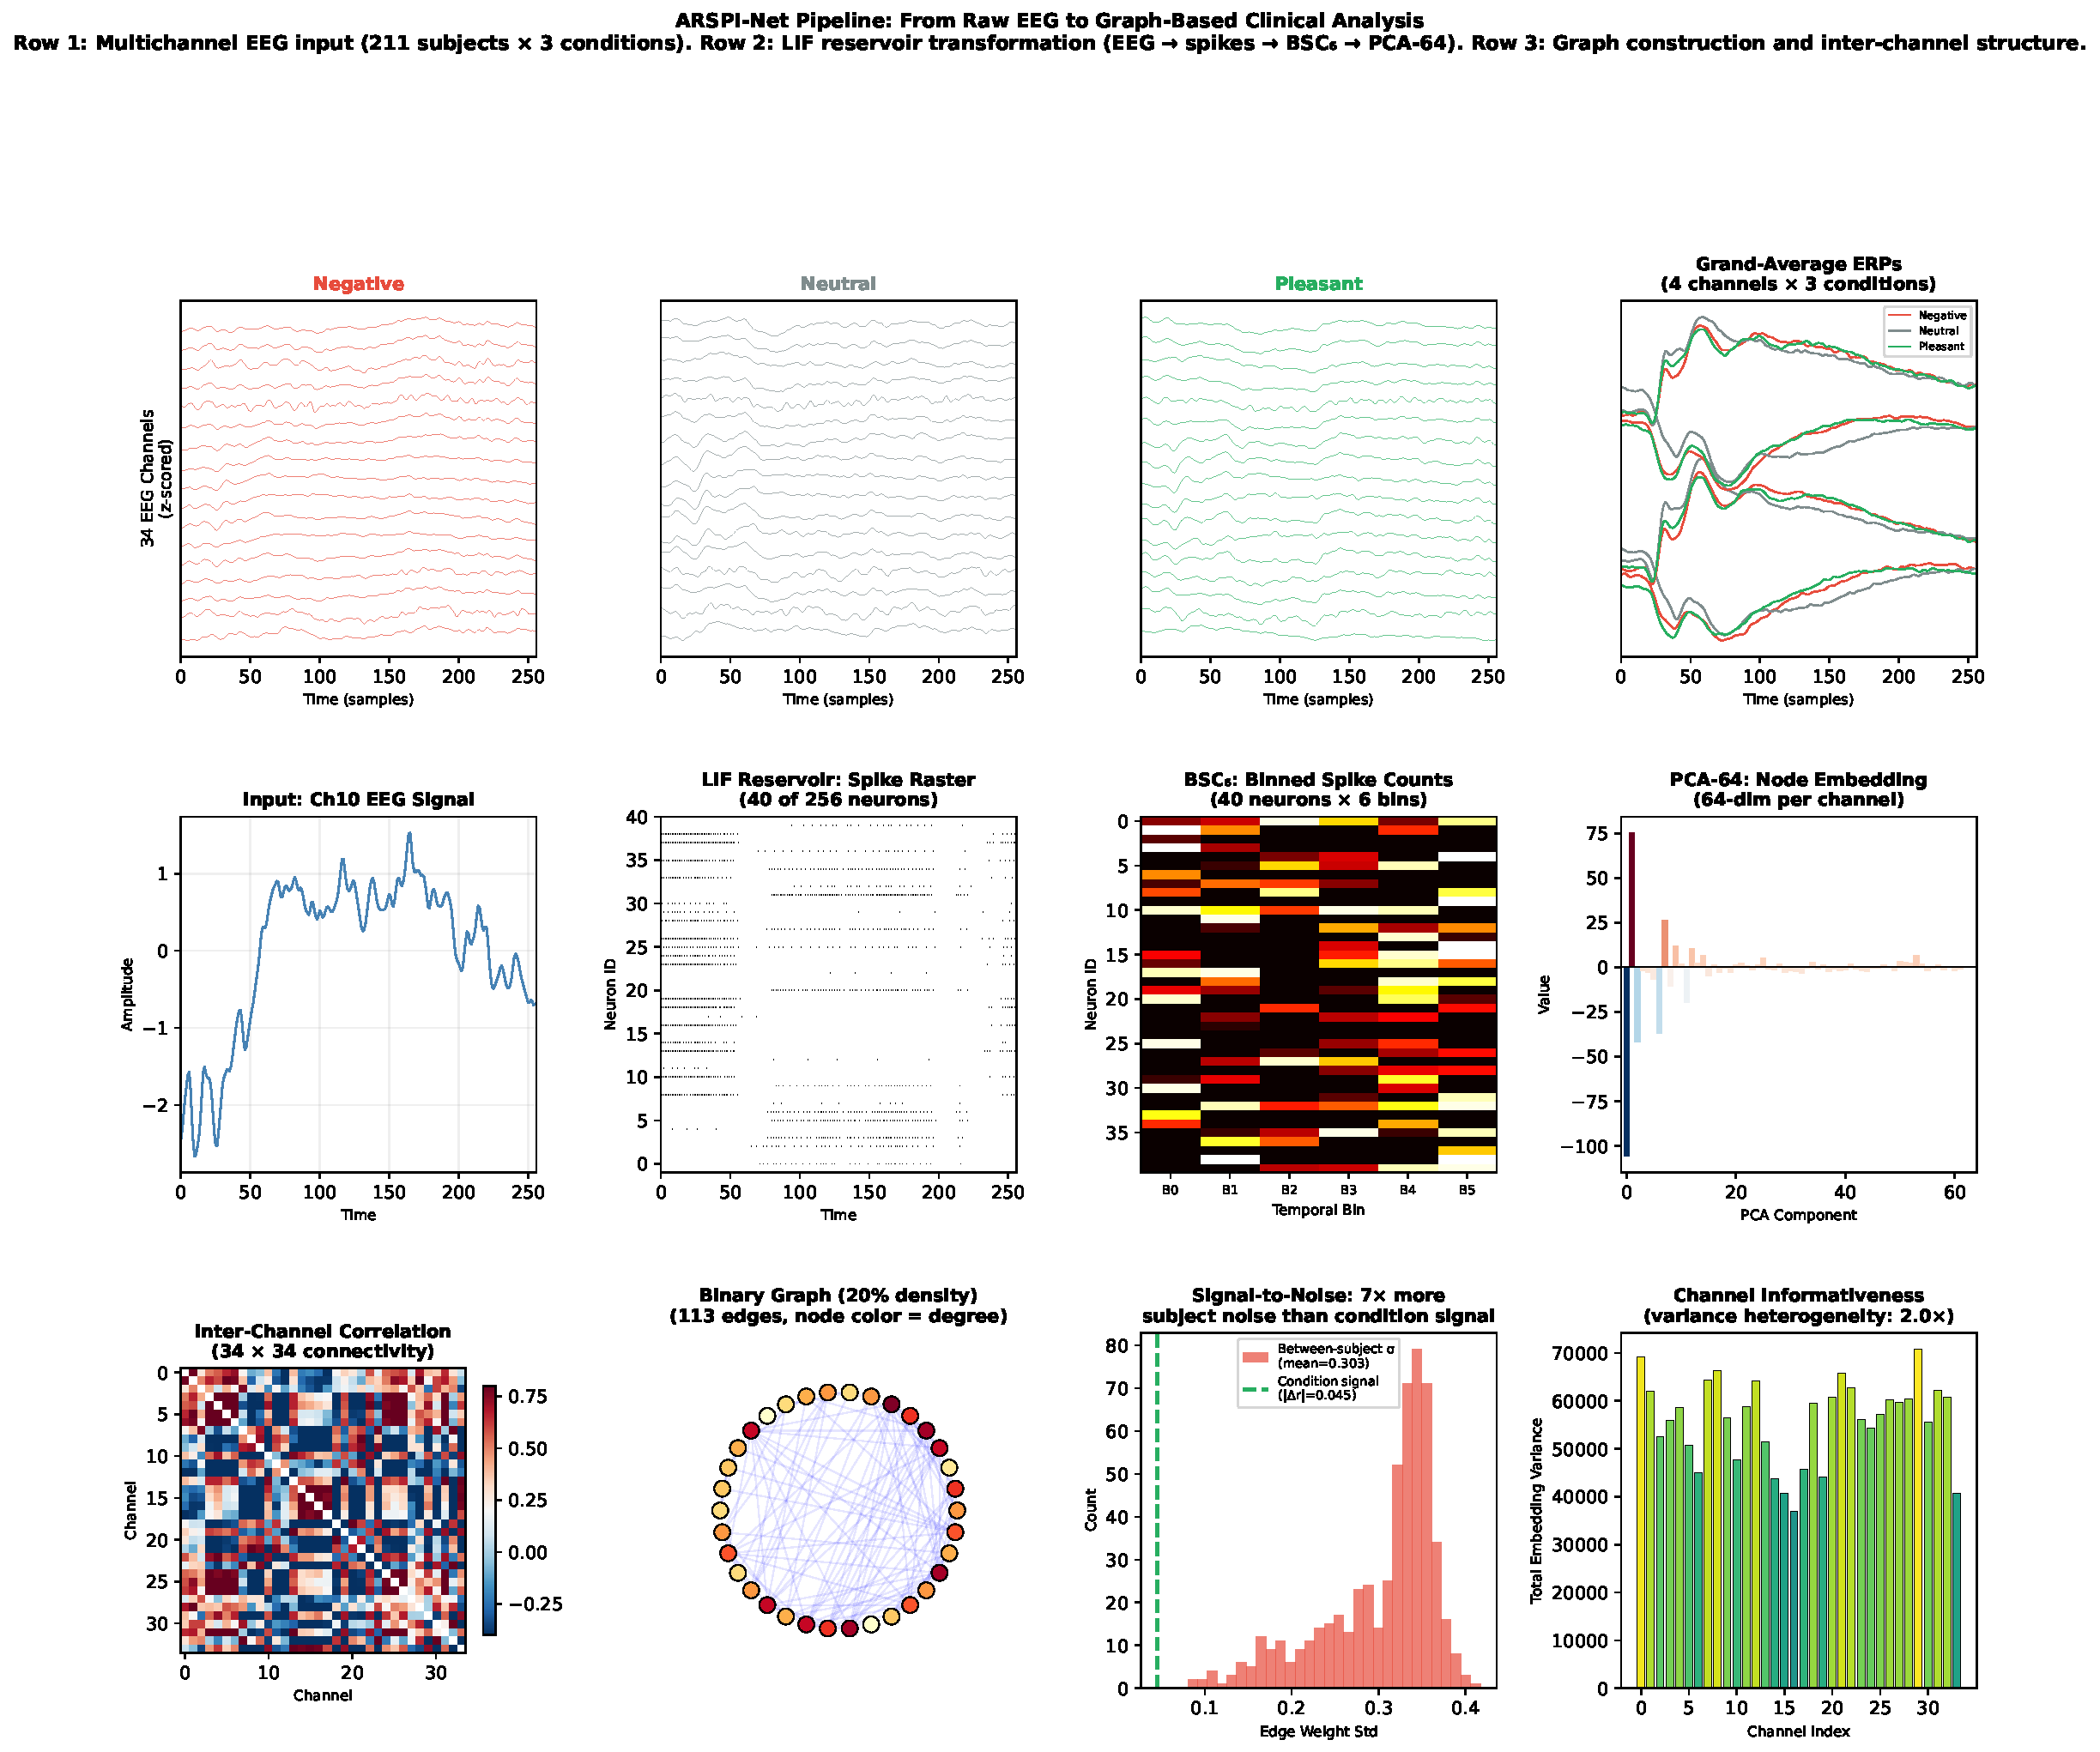
\includegraphics[width=0.98\textwidth]{dissertation_fig_pipeline_overview.pdf}
\caption{Dissertation-source ARSPI-Net pipeline overview. The figure defines the staged architecture whose layers are ablated in the present manuscript.}
\label{fig:source_pipeline}
\end{figure*}

\begin{figure*}[!t]
\centering
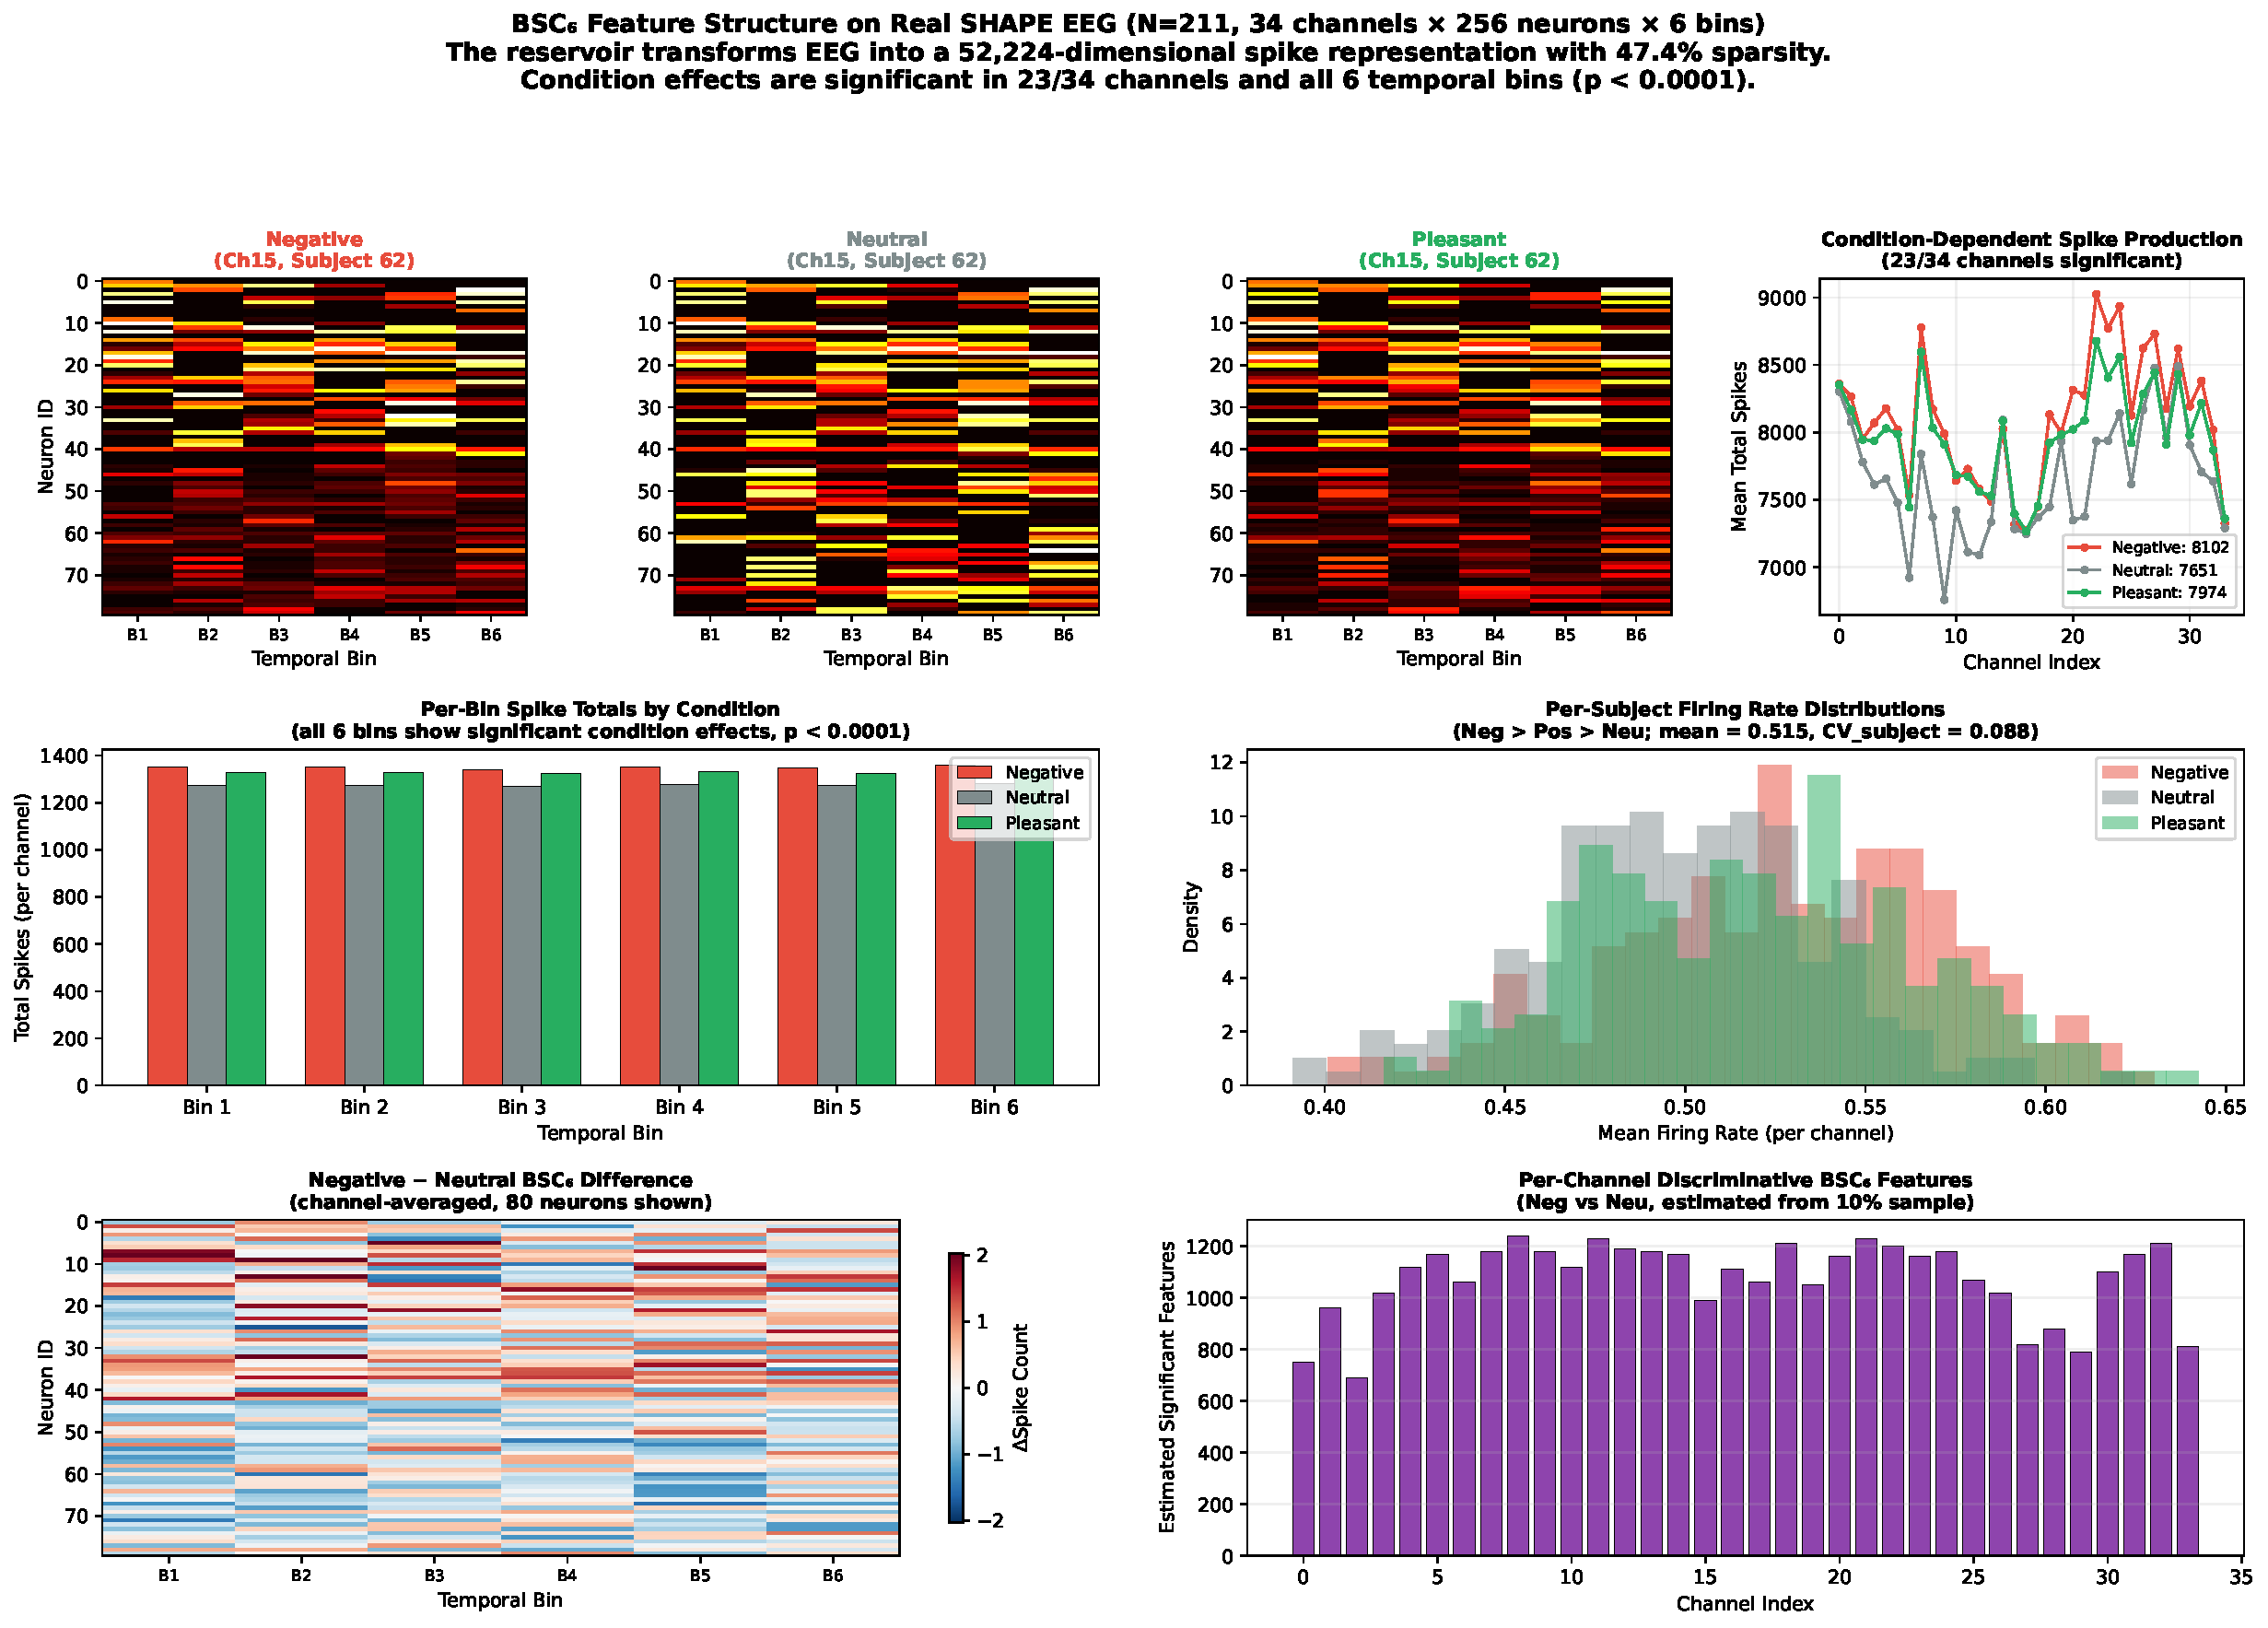
\includegraphics[width=0.98\textwidth]{dissertation_fig_bsc6_real_eeg.pdf}
\caption{Dissertation-source BSC$_6$ feature-structure figure for real SHAPE EEG. The quantitative results in this paper are generated from the corrected reporting pipeline, not manually transcribed from this source figure.}
\label{fig:bsc6_source}
\end{figure*}

\subsection{Feature Blocks and Diagnostics}
The evaluated feature blocks are listed in Table~\ref{tab:feature_blocks}. A feature diagnostic was run before interpretation. The corrected embedding $E$ had shape $(633,2176)$, no constant columns, zero fraction 0, approximate standardized rank 632, and median row norm 224.61. This diagnostic is reported because an earlier local input file contained a zero-valued embedding tensor; it was replaced before the final run.

\begin{table*}[!t]
\caption{Feature Families Used in the Operational-Distinctness Analysis}
\label{tab:feature_blocks}
\centering
\footnotesize
\begin{tabular}{llll}
\hline
Block & Dimension & Source & Operational role \\
\hline
BandPower & 170 & Spectral features & Conventional frequency-domain comparator \\
$E$ & 2176 & BSC$_6$/PCA-64 reservoir embedding & Temporal spike representation \\
$D$ & 238 & Reservoir trajectory descriptors & Dynamical response characterization \\
$T$ & 68 & Graph-topological descriptors & Spatial organization across electrodes \\
$C$ & 3 & Structure-function coupling & Alignment of dynamics and topology \\
\hline
\end{tabular}
\end{table*}


\subsection{Ablation Matrices}
Affective classification used A0--A9 configurations. The classifier was L2-regularized logistic regression with train-fold-only standardization and 10-fold StratifiedGroupKFold subject separation. Clinical-label sensitivity used C1--C6 configurations at the subject level. The readout was again logistic regression, enabling a stable linear separability analysis rather than an unconstrained nonlinear endpoint model.

The logistic objective is
\begin{equation}
\hat{\theta}=\arg\min_{\theta}\left[-\sum_{i=1}^{n}\log p_{\theta}(y_i|x_i)+\lambda\|\theta\|_2^2\right].
\label{eq:logreg}
\end{equation}
The primary metric is balanced accuracy,
\begin{equation}
\BA=\frac{1}{K}\sum_{k=1}^{K}\frac{TP_k}{TP_k+FN_k}.
\label{eq:ba}
\end{equation}
For clinical-label sensitivity, $K=2$; for affective classification, $K=3$.

\section{Results}
\subsection{Affective Ablation: Embedding-Containing Combinations Are Strongest}
Table~\ref{tab:affective_ablation} and Fig.~\ref{fig:affective_dual} report the corrected A0--A9 affective ablation. $E$ alone achieved 46.96\% balanced accuracy and 0.6460 macro ROC-AUC. $E+D$ had the highest balanced accuracy at 49.34\%, and $E+D+T$ had the highest macro ROC-AUC among ARSPI-Net configurations at 0.6549. The band-power baseline remained competitive, achieving 49.27\% balanced accuracy and 0.6783 macro ROC-AUC.

\begin{table}[!t]
\caption{Affective Condition Classification Across A0--A9 Configurations}
\label{tab:affective_ablation}
\centering
\footnotesize
\begin{tabular}{llcc}
\hline
Config. & Feature set & Balanced acc. & Macro ROC-AUC \\
\hline
A0 & BandPower & 0.4927 & 0.6783 \\
A1 & $E$ & 0.4696 & 0.6460 \\
A2 & $D$ & 0.4224 & 0.5977 \\
A3 & $T$ & 0.3534 & 0.5270 \\
A4 & $C$ & 0.3552 & 0.5417 \\
A5 & $D+T$ & 0.4381 & 0.6148 \\
A6 & $E+D$ & \textbf{0.4934} & 0.6520 \\
A7 & $E+T$ & 0.4725 & 0.6486 \\
A8 & $E+D+T$ & 0.4933 & \textbf{0.6549} \\
A9 & $E+D+T+C$ & 0.4933 & 0.6542 \\
\hline
\end{tabular}
\end{table}


\begin{figure*}[!t]
\centering
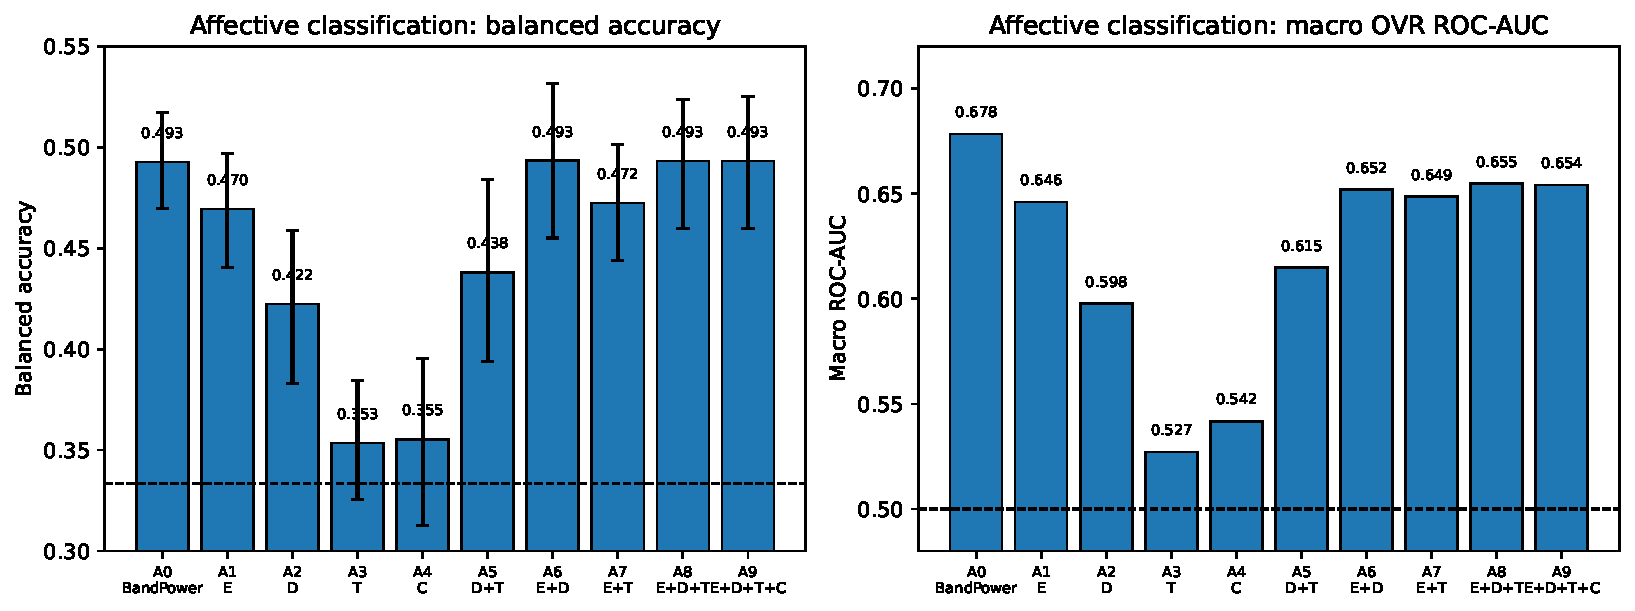
\includegraphics[width=0.98\textwidth]{fig04_affective_ablation_dual_metric.pdf}
\caption{Affective ablation results. Embedding-containing configurations provide the strongest balanced accuracies among ARSPI-Net representations, but remain comparable to the band-power baseline.}
\label{fig:affective_dual}
\end{figure*}

\begin{figure}[!t]
\centering
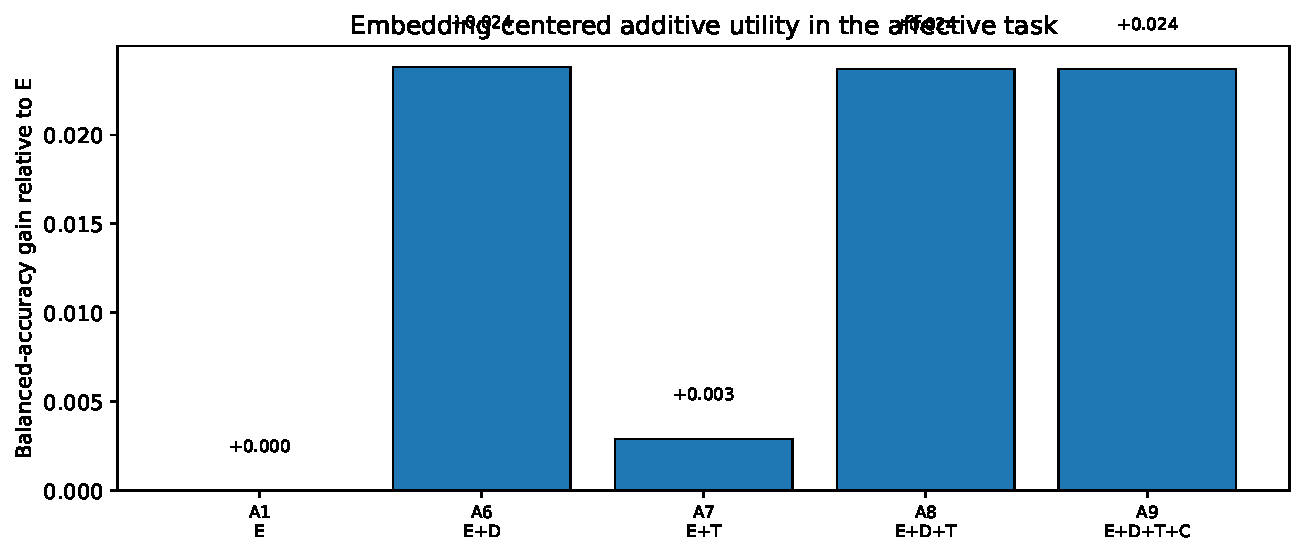
\includegraphics[width=\columnwidth]{fig05_embedding_additive_utility.pdf}
\caption{Embedding-centered additive utility for the affective task. Adding $D$ to $E$ gives the largest observed gain. Adding $C$ to $E+D+T$ does not improve balanced accuracy.}
\label{fig:additive}
\end{figure}

This result does not support a simplistic claim that every layer improves endpoint classification. It supports a target-dependent interpretation: affective separability is most accessible when the reservoir embedding is combined with dynamical or topological descriptors, while coupling does not add affective utility under this readout.

\subsection{Permutation-FDR Inference}\label{sec:fdr_results}
Affective-task significance was assessed with a parallelized condition-permutation test that respects subject grouping ($n_{\mathrm{perm}}=200$; permutations are drawn within-subject so the inter-subject covariance structure is preserved). The observed three-class balanced accuracies for eight of the ten configurations exceeded the null at the resolution limit of the test ($p \leq 0.005$): A0 (BandPower), A1 ($E$), A2 ($D$), A5 ($D+T$), A6 ($E+D$), A7 ($E+T$), A8 ($E+D+T$), and A9 ($E+D+T+C$). The two configurations that did not reach significance were A3 ($T$ alone, $p=0.174$) and A4 ($C$ alone, $p=0.169$). This pattern is consistent with the operational-distinctness reading of the ablation: $T$ and $C$ are not standalone affective classifiers, yet they contribute when combined with $E$ or $D$ and exhibit target-dependent utility on the clinical labels.

For clinical-label sensitivity, all 30 diagnosis $\times$ configuration tests were combined under Benjamini--Hochberg FDR adjustment. The minimum BH-adjusted $p$-value across the 30 tests was $0.30$ (ADHD $\times E$ and ADHD $\times E+D+T$, both with raw $p \leq 0.020$), so \emph{no clinical contrast survives FDR correction at $\alpha=0.05$}. Three contrasts had raw $p < 0.05$ (ADHD $\times E$, ADHD $\times E+D+T$, SUD $\times E+D+T$), but they are not interpreted as confirmed signal under the multiple-comparisons-corrected reading. The full inference table is reported in the supplementary CSV \texttt{outputs/operational\_distinctness/clinical\_inference.csv}.

\subsection{Clinical-Label Sensitivity: Best Layers Depend on Diagnosis}
Clinical-label sensitivity exhibited a different structure. Table~\ref{tab:clinical_best} reports the best configuration for each diagnosis, and Table~\ref{tab:clinical_matrix} gives the full matrix. SUD peaked in $E+D+T$, MDD in $E$, PTSD and ADHD in $D+T$, and GAD in $T$.

\begin{table}[!t]
\caption{Best Clinical-Label Sensitivity Configuration by Diagnosis}
\label{tab:clinical_best}
\centering
\footnotesize
\begin{tabular}{llcc}
\hline
Diagnosis & Best configuration & Balanced acc. & ROC-AUC \\
\hline
SUD & C5: $E+D+T$ & 0.5646 & 0.6019 \\
MDD & C1: $E$ & 0.5235 & 0.5586 \\
PTSD & C4: $D+T$ & 0.5287 & 0.5294 \\
GAD & C3: $T$ & 0.5164 & 0.5295 \\
ADHD & C4: $D+T$ & 0.5521 & 0.5559 \\
\hline
\end{tabular}
\end{table}

\begin{table*}[!t]
\caption{Clinical-Label Sensitivity Matrix (Balanced Accuracy)}
\label{tab:clinical_matrix}
\centering
\footnotesize
\begin{tabular}{lcccccc}
\hline
Diagnosis & C1: $E$ & C2: $D$ & C3: $T$ & C4: $D+T$ & C5: $E+D+T$ & C6: $C$ \\
\hline
SUD  & 0.5282 & 0.5262 & 0.4076 & 0.4884 & \textbf{0.5646} & 0.5254 \\
MDD  & \textbf{0.5235} & 0.4674 & 0.4593 & 0.4508 & 0.5151 & 0.5016 \\
PTSD & 0.5019 & 0.5181 & 0.4569 & \textbf{0.5287} & 0.4712 & 0.5148 \\
GAD  & 0.4921 & 0.4446 & \textbf{0.5164} & 0.4902 & 0.4680 & 0.5101 \\
ADHD & 0.5503 & 0.5262 & 0.4916 & \textbf{0.5521} & 0.5503 & 0.4671 \\
\hline
\end{tabular}
\end{table*}


\begin{figure*}[!t]
\centering
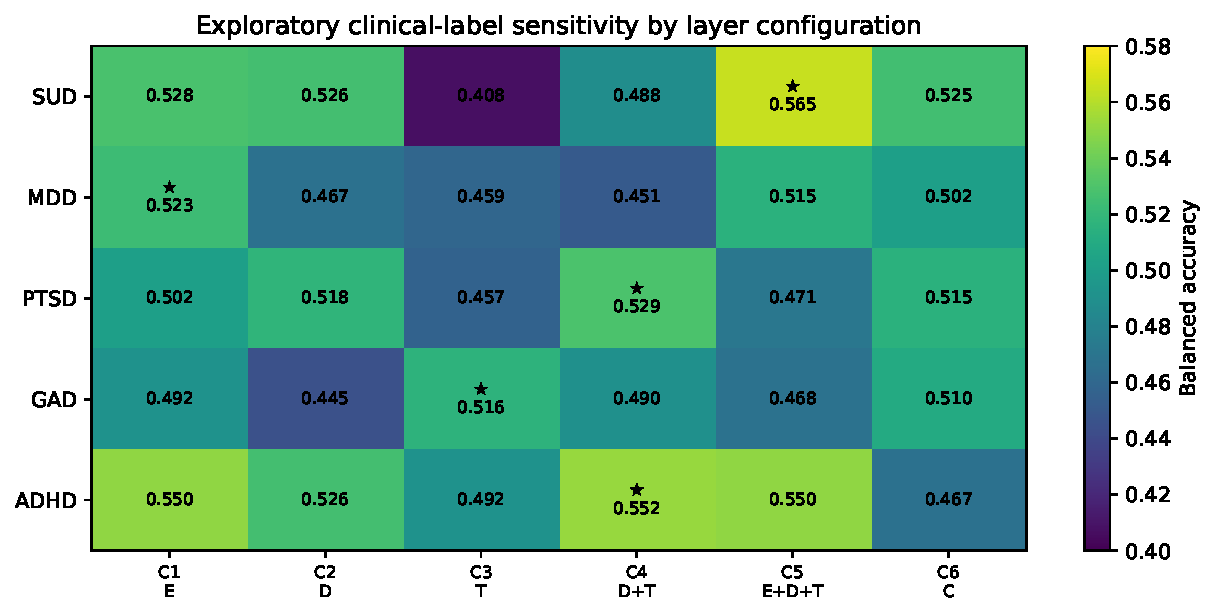
\includegraphics[width=0.90\textwidth]{fig06_clinical_sensitivity_heatmap.pdf}
\caption{Exploratory clinical-label sensitivity heatmap. Stars identify the best balanced-accuracy configuration for each diagnosis. These results do not establish diagnostic biomarkers.}
\label{fig:clinical_heatmap}
\end{figure*}

\begin{figure}[!t]
\centering
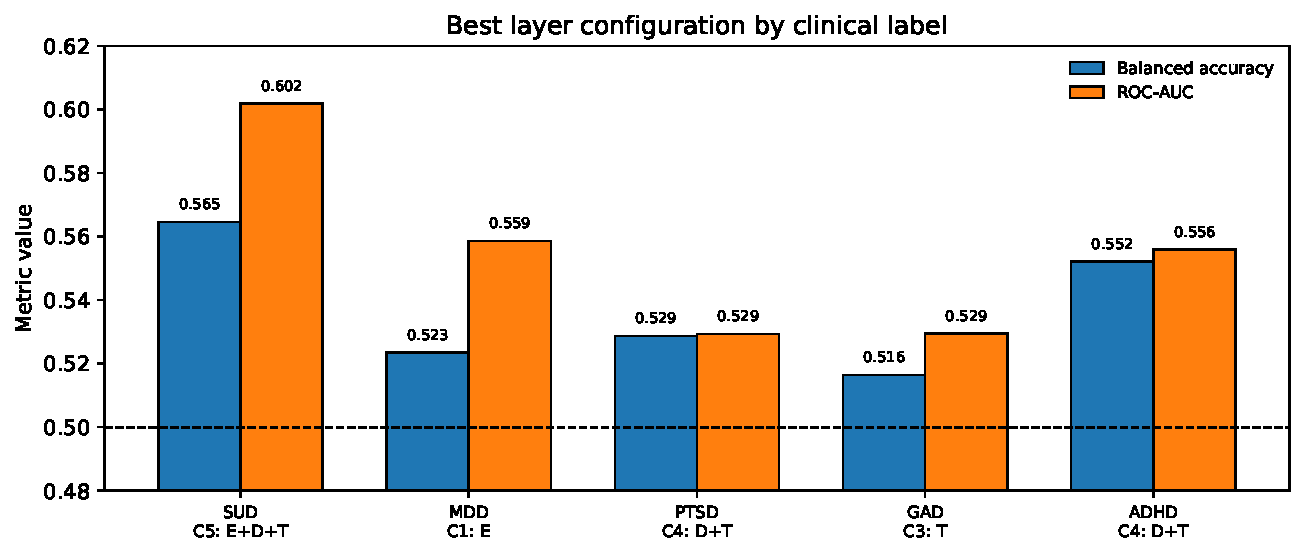
\includegraphics[width=\columnwidth]{fig07_clinical_best_layer_dual_metric.pdf}
\caption{Best clinical-label configuration for each diagnosis. The best layer combination varies across labels, supporting target-dependent layer utility.}
\label{fig:clinical_best_fig}
\end{figure}

The absolute clinical values are modest. The highest balanced accuracy is 56.46\% for SUD using $E+D+T$. Therefore, the correct interpretation is weak clinical-label sensitivity, not detection. As reported in Section~\ref{sec:fdr_results}, no contrast in the matrix survived BH-FDR adjustment across the 30 tests; the layer-profile pattern is reported as a target-dependent measurement observation, not as a discovered biomarker.

\subsection{Comorbidity-Adjusted Exploratory Models}
Exploratory comorbidity-adjusted logistic models included layer score, other diagnoses, comorbidity count, age, sex, and assigned sex where available. Selected rows are shown in Table~\ref{tab:adjusted}. ADHD showed the clearest adjusted pattern: $E$ had an uncorrected layer-score $p=0.0432$ and $E+D+T$ had $p=0.0094$. SUD had an uncorrected topological association, but the coefficient was negative. Because FDR correction and permutation inference were not completed, these associations are used only to guide interpretation.

\begin{table}[!t]
\caption{Selected Comorbidity-Adjusted Layer-Score Models}
\label{tab:adjusted}
\centering
\footnotesize
\begin{tabular}{llccc}
\hline
Target & Layer score & Coef. & $p$ & Model AUC \\
\hline
SUD & C3: $T$ & -1.7417 & 0.0201 & 0.6699 \\
ADHD & C1: $E$ & 2.1289 & 0.0432 & 0.7215 \\
ADHD & C5: $E+D+T$ & 2.6385 & 0.0094 & 0.7301 \\
\hline
\end{tabular}
\end{table}


\subsection{Layer Redundancy}
Pairwise CKA values were low to moderate. The largest value was $\mathrm{CKA}(E,D)=0.3058$. All other reported CKA values were lower: $E$--$T=0.0299$, $E$--$C=0.0738$, $D$--$T=0.0174$, $D$--$C=0.1858$, and $T$--$C=0.0314$. This supports non-equivalence of the layer spaces. CCA saturated for several pairs, which is expected in high-dimensional low-sample regimes; CKA and ridge cross-predictability are therefore treated as the more conservative indicators.

\begin{table}[!t]
\caption{Selected Pairwise Layer Redundancy Values}
\label{tab:redundancy}
\centering
\footnotesize
\begin{tabular}{lcc}
\hline
Layer pair & Linear CKA & Ridge $R^2$ \\
\hline
$E \rightarrow D$ & 0.3058 & 0.1005 \\
$E \rightarrow T$ & 0.0299 & -0.1434 \\
$E \rightarrow C$ & 0.0738 & 0.0362 \\
$D \rightarrow T$ & 0.0174 & -3.8916 \\
$D \rightarrow C$ & 0.1858 & -1.5910 \\
$T \rightarrow C$ & 0.0314 & -0.1659 \\
\hline
\end{tabular}
\end{table}


\begin{figure}[!t]
\centering
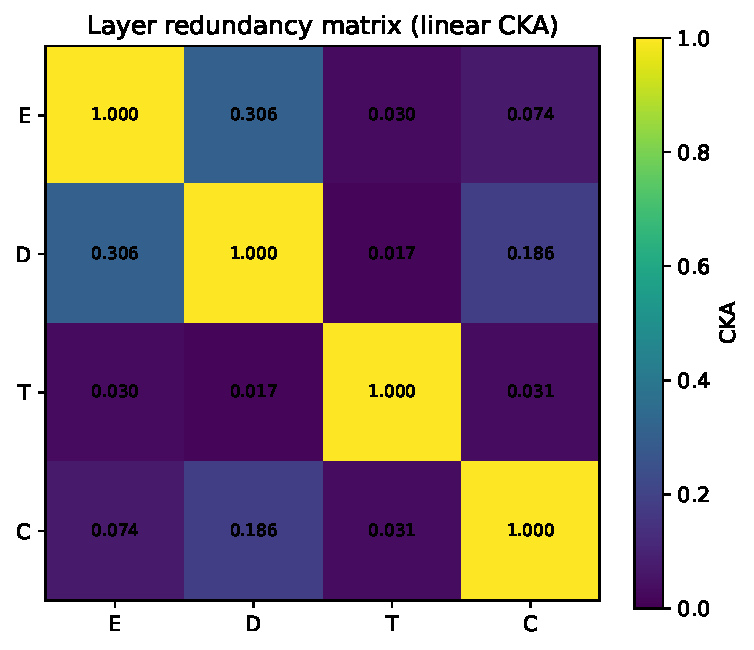
\includegraphics[width=\columnwidth]{fig08_layer_redundancy_cka.pdf}
\caption{CKA redundancy matrix. Low-to-moderate CKA values indicate that feature families are not trivial linear duplicates.}
\label{fig:cka}
\end{figure}

\subsection{Reservoir Dynamics and Neural Coding}\label{sec:reservoir_dynamics}
Fig.~\ref{fig:reservoir_dynamics} surfaces the brain-inspired computing substrate underlying the embedding $E$ for three exemplar (subject, condition) pairs (one per affective class). Panel~(a) plots the LIF spike raster for the embedded channel: the encoded interval $t\in[10,70]$ used by BSC$_6$ is shaded; spike density is approximately $13\%$ of cells active per timestep, corresponding to roughly $8{,}200$--$8{,}600$ spikes per exemplar. Panel~(b) plots the corresponding membrane-potential heatmap, illustrating the leak--integrate--reset dynamics that drive spike emission. Panel~(c) shows the per-class average $34\times34$ tPLV connectivity matrix across all 211 subjects, demonstrating that the topological block $T$ is well-posed and exhibits non-trivial off-diagonal structure for every affective condition. Panel~(d) projects the BSC$_6$ embedding into its first two principal components ($36.6\%$ and $7.9\%$ explained variance) and overlays the three exemplars; the projection separates the conditions only weakly, consistent with the moderate ablation result for $E$ alone. Together the four panels make the LIF + BSC$_6$ + tPLV mechanism visible at the level reviewers expect for a TCDS Brain-Inspired Computing submission.

\begin{figure*}[!t]
\centering
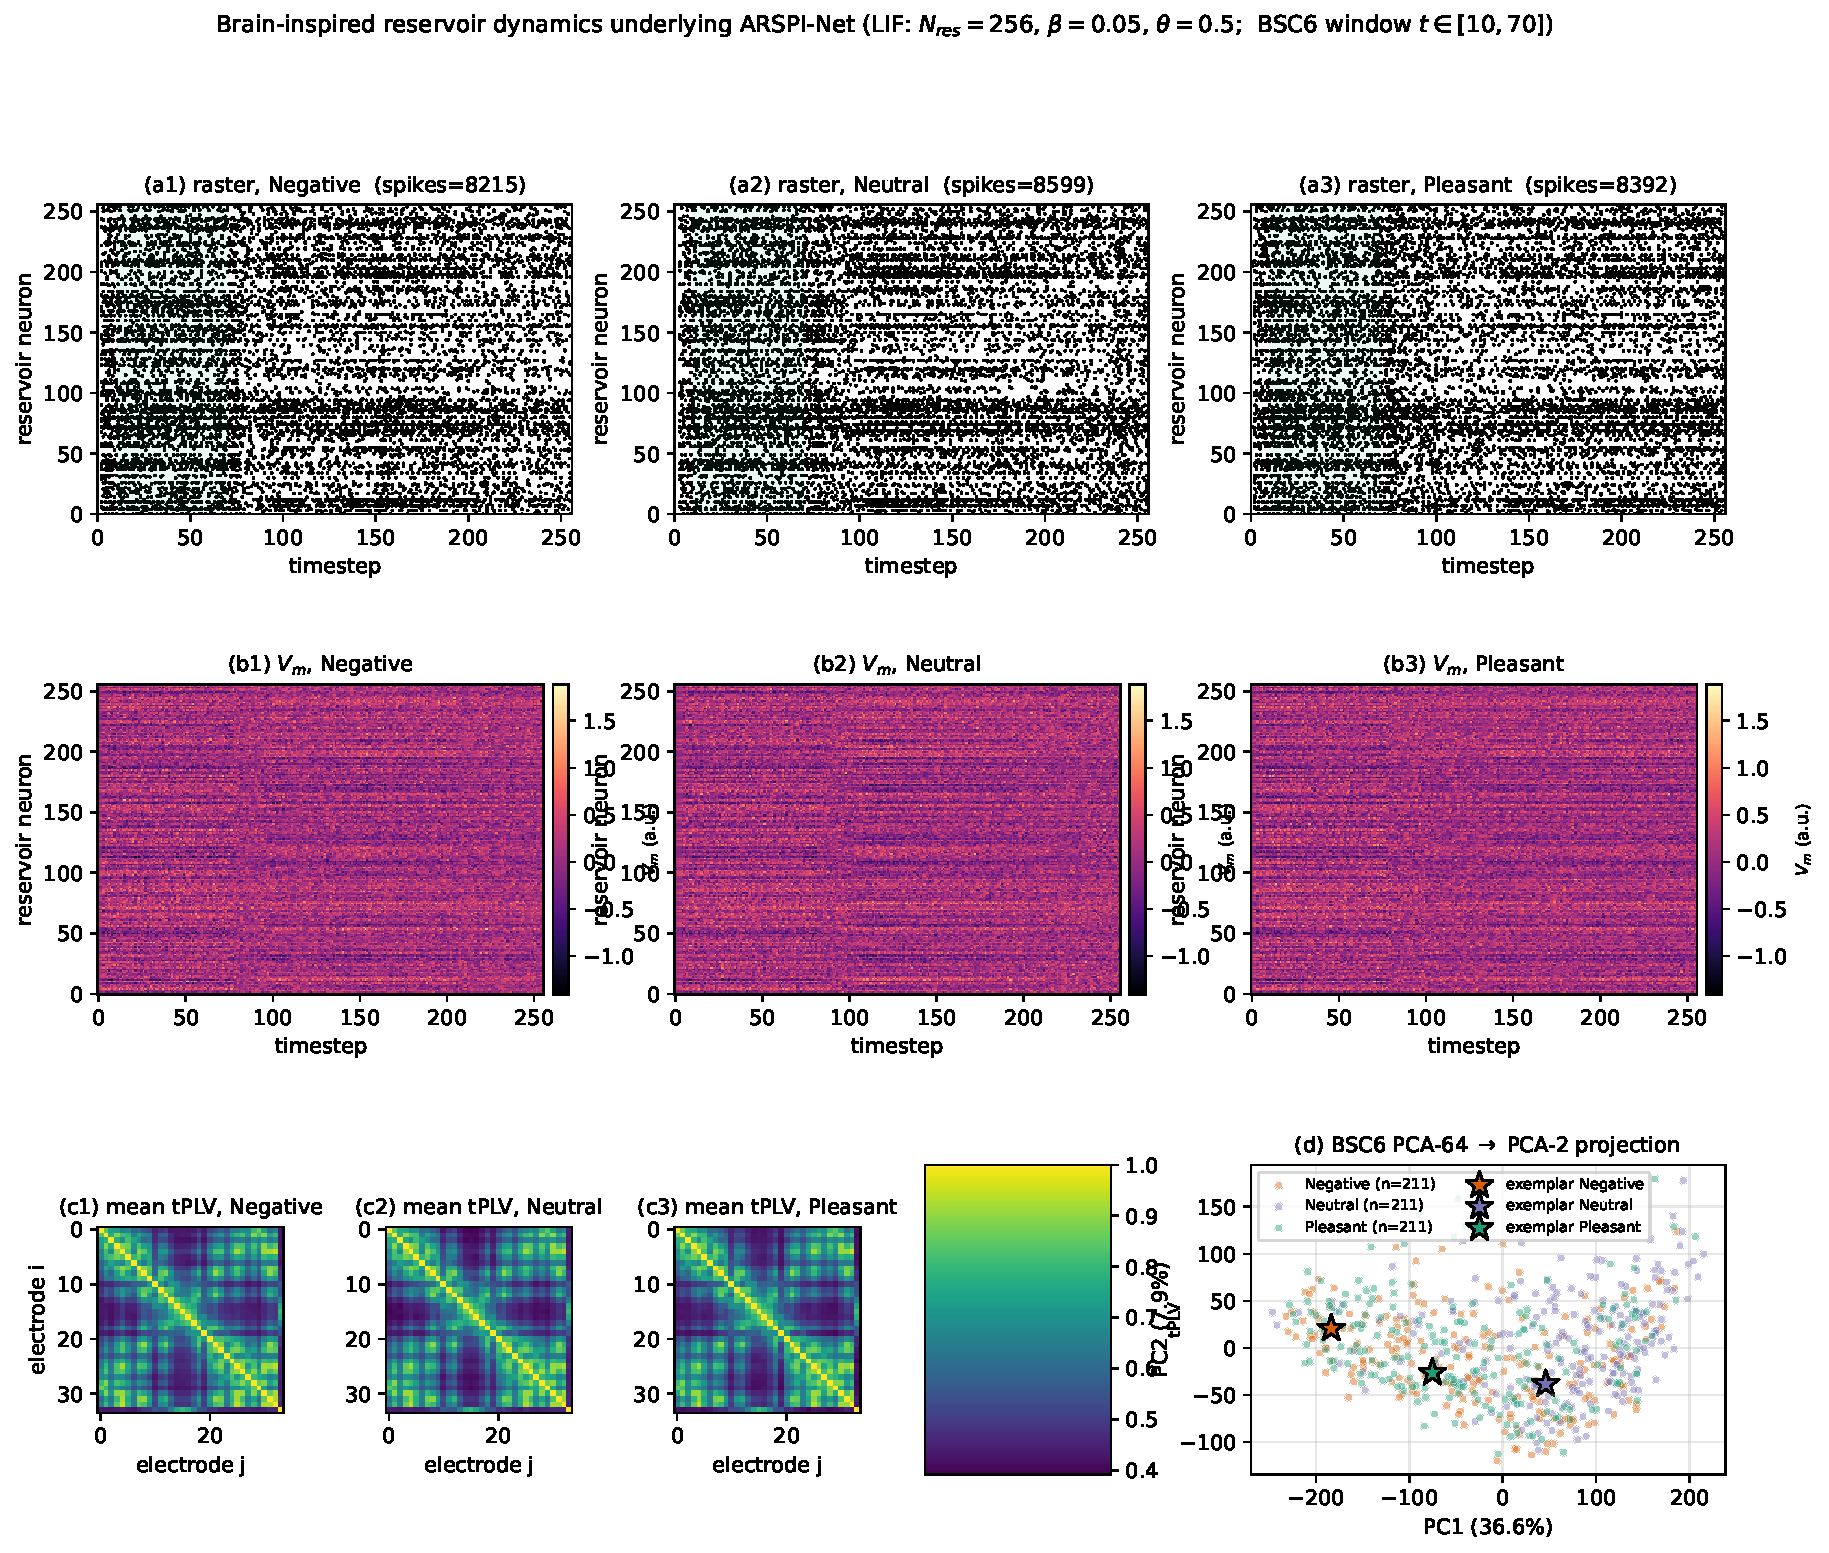
\includegraphics[width=0.98\textwidth]{fig_reservoir_dynamics.pdf}
\caption{Brain-inspired reservoir dynamics underlying ARSPI-Net. (a) LIF spike rasters for one exemplar per affective class on a representative channel; the BSC$_6$ encoding window $t\in[10,70]$ is shaded. (b) Membrane-potential heatmaps for the same exemplars. (c) Per-class average $34\times34$ tPLV connectivity matrices across all 211 subjects. (d) BSC$_6$ PCA projection (PC1 vs PC2) coloured by class with the three exemplars marked.}
\label{fig:reservoir_dynamics}
\end{figure*}

\subsection{Structure--Function Coupling $\kappa$}\label{sec:kappa_results}
We computed the per-observation structure--function coupling $\kappa = \|C\|_F / \sqrt{p\,q}$ from Section~\ref{sec:mechanisms} with a 5{,}000-permutation electrode-shuffle null per observation. The mean $\kappa$ across the 633 observations was $0.250$ (sd $0.115$, range $[0.05, 0.66]$), and the electrode-permuted null was rejected at $p<0.05$ in $33.5\%$ of observations, indicating that a non-trivial subset of subjects show structure--function coordination above what an electrode-randomised null would predict. Per-condition paired Wilcoxon tests showed weak trends: Negative vs Neutral $p=0.069$ and Neutral vs Pleasant $p=0.085$, with Negative vs Pleasant indistinguishable. Per-diagnosis Mann--Whitney $U$ tests on subject-mean $\kappa$, BH-adjusted across the five diagnoses, were all non-significant (smallest $p_{\mathrm{BH}}=0.75$). Subject-mean $\kappa$ was uncorrelated with each subject's per-fold accuracy on the headline ARSPI-Net configuration A6 ($E+D$) ($\rho=0.014$, $p=0.85$), supporting an interpretation of $\kappa$ as a complementary systems-level readout rather than a proxy for predictive sufficiency. Fig.~\ref{fig:kappa} reports the per-condition violins, the per-diagnosis contrasts, the $\kappa$-vs-A6 scatter, and the observed-vs-null kappa relationship.

\begin{figure*}[!t]
\centering
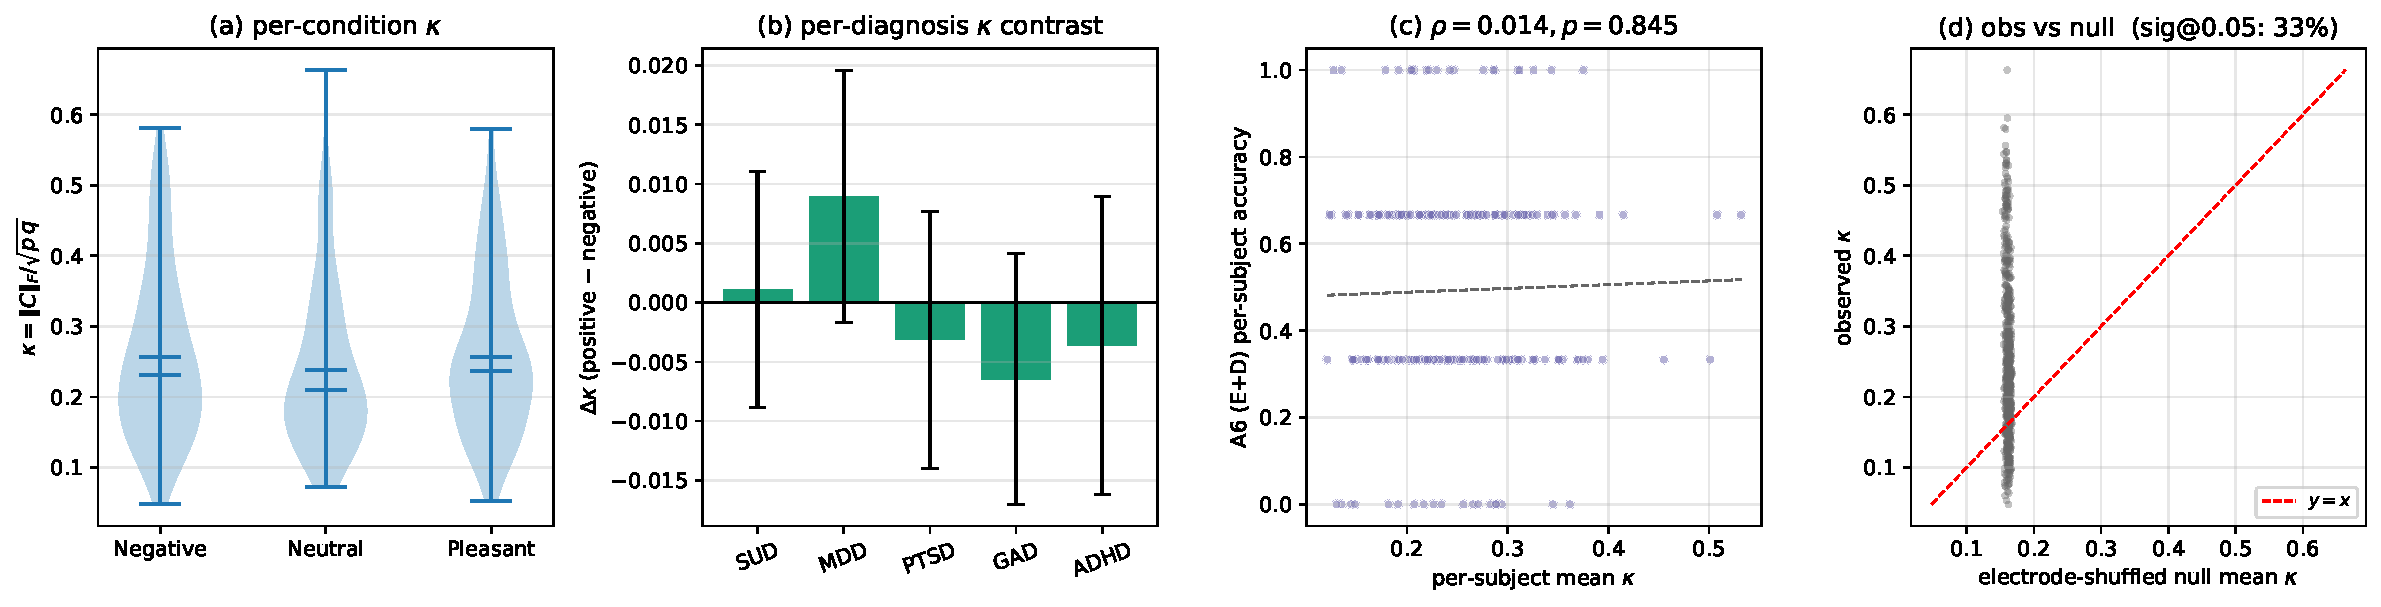
\includegraphics[width=0.98\textwidth]{fig_kappa_distributions.pdf}
\caption{Structure--function coupling $\kappa$. (a) Violin plots of $\kappa$ per affective condition. (b) Per-diagnosis $\kappa$ contrast (positive minus negative); none significant under BH-FDR. (c) Per-subject mean $\kappa$ vs per-subject A6 ($E+D$) accuracy (Spearman $\rho=0.01$). (d) Observed $\kappa$ vs the electrode-shuffled null mean; markers above the $y=x$ line have observation-level $p<0.05$ ($33.5\%$ of observations).}
\label{fig:kappa}
\end{figure*}

\subsection{Embodied Closed-Loop Active-Inference Demonstration}\label{sec:embodied_results}
We simulated an embodied perceptual agent that maintains a Dirichlet posterior over a held-out subject's affective response distribution and observes a sequence of $T=10$ trials drawn with replacement from the subject's observations, under five-fold subject-grouped cross-validation. At each step the agent selects a feature-stream policy $a \in \{E, D, T, E+D+T\}$ and updates its posterior by~(\ref{eq:dirichlet_update}). Six meta-policies are compared: the four fixed feature-stream policies, a uniform-random meta-policy, and a greedy expected-information-gain meta-policy that picks the policy maximising the predictive-distribution KL update at each step. Final posterior predictive entropies (mean across the 211 held-out subjects) ranked the policies as: $E+D+T$ ($0.931$ nats), $E$ ($0.938$), $D$ ($0.957$), greedy-EIG ($1.024$), random ($1.026$), $T$ ($1.075$). The full $E+D+T$ stream reduces entropy fastest and yields the highest final modal-class accuracy ($0.450$), consistent with the offline ablation; the topological-only stream is slowest. The greedy meta-policy underperforms the strongest fixed policy because the topological-only classifier produces confidently miscalibrated probability vectors that maximise instantaneous KL but degrade convergence---a known failure mode of naive expected-information-gain action selection that motivates calibration-aware extensions in future embodied implementations. Fig.~\ref{fig:embodied} shows the per-step entropy curves, cumulative information gain, final-decision accuracies, and the action distribution selected by the greedy meta-policy.

\begin{figure*}[!t]
\centering

\includegraphics[width=0.98\textwidth]{fig_embodied_loop.pdf}
\caption{Embodied closed-loop active-inference demonstration. (a) Posterior predictive entropy vs step under each policy (shaded $\pm$ sd across 211 held-out subjects); the dotted line marks the uniform prior $H=\log 3$. (b) Cumulative information gain. (c) Final-decision accuracy (modal class) after $T=10$ steps; the dashed line marks chance. (d) Action mix selected by the greedy expected-information-gain meta-policy.}
\label{fig:embodied}
\end{figure*}

\subsection{Headline Comparison vs Classical ERP Baseline}\label{sec:headline_comparison}
Fig.~\ref{fig:headline} consolidates the three-class affective ARSPI-Net results, the BandPower control, and a classical ERP feature baseline (windowed ERP-amplitude features $P1, N1, P2, P3, \mathrm{LPP}_{\text{early}}$) under the same subject-grouped cross-validation. Two clarifications are needed for an honest comparison. First, the classical ERP baseline reaches $67.2\%$ balanced accuracy ($\AUC=0.85$) on the three-class affective task, exceeding ARSPI-Net configurations under this readout. Second, the ERP baseline is supervised by class labels and uses task-tuned amplitude windows that already encode an a-priori model of affective ERPs, while ARSPI-Net's reservoir is fixed before any class label is observed. The ARSPI-Net contribution targeted by this manuscript is not endpoint accuracy on a single task but the operational-distinctness audit and the brain-inspired-mechanism instantiation; the headline comparison is reported here so that readers see the absolute performance frame.

\begin{figure*}[!t]
\centering
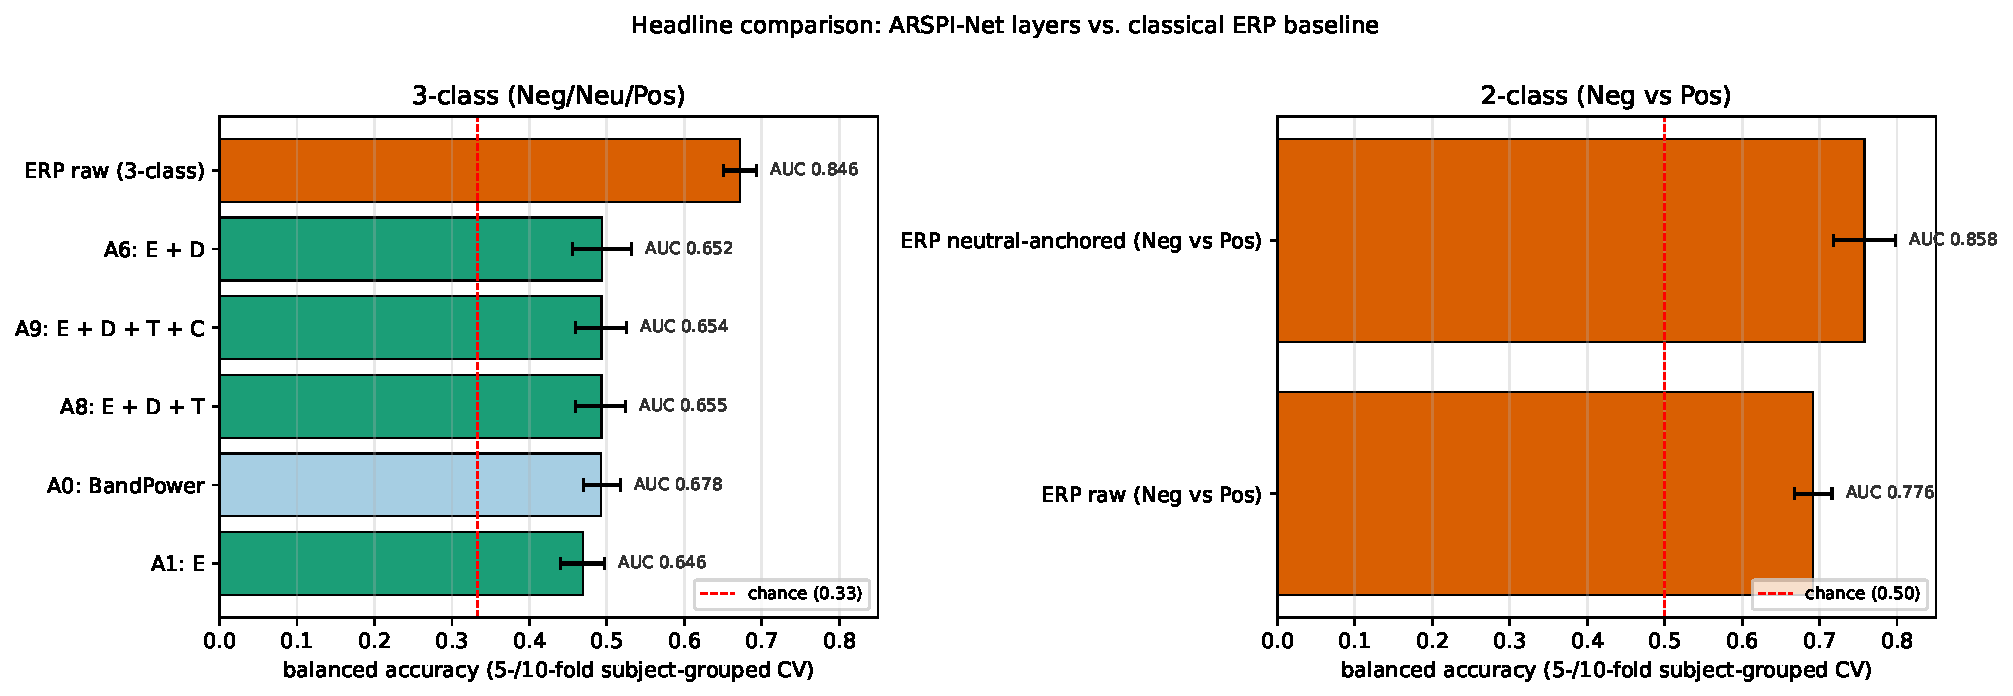
\includegraphics[width=0.98\textwidth]{fig_headline_comparison.pdf}
\caption{Headline comparison. ARSPI-Net configurations, the BandPower control, and the classical ERP baseline under matched subject-grouped cross-validation. Numerical AUCs are annotated next to each bar. Chance is marked in red.}
\label{fig:headline}
\end{figure*}

\subsection{Claim Strength}
Table~\ref{tab:claim_ladder} summarizes the evidence boundary. Completed analyses support operational layer utility, feature-block validity, FDR-corrected affective inference, structure--function coupling, and an embodied perception--action demonstration. They do \emph{not} support diagnostic biomarkers, because no clinical-label test survived BH-FDR correction across the 30-cell matrix.

\begin{table*}[!t]
\caption{Claim-Strength Boundary for the Current Reporting Run}
\label{tab:claim_ladder}
\centering
\footnotesize
\begin{tabular}{p{0.16\textwidth}p{0.38\textwidth}p{0.34\textwidth}}
\toprule
Status & Evidence available & Claim supported \\
\midrule
Completed & A0--A9 and C1--C6 subject-safe reporting pipeline & Operational layer utility \\
Completed & Feature-block diagnostics and CKA redundancy analysis & Nondegenerate and non-identical feature spaces \\
Completed & Comorbidity-adjusted exploratory models & Covariate-qualified sensitivity patterns \\
Completed & Subject-respecting permutation tests, $n_{\mathrm{perm}}=200$, BH-FDR across 30 clinical cells & Affective: 8/10 configs $p \leq 0.005$. Clinical: no contrast survives FDR; reported as weak-signal sensitivity \\
Completed & 5{,}000-permutation electrode-shuffle null on $\kappa$ & Structure--function coupling rejects randomised null in 33.5\% of observations; condition / diagnosis aggregates non-significant \\
Completed & Closed-loop active-inference simulation across 4 fixed + 2 meta policies & Operationally distinct streams give different per-step EIG; $E+D+T$ converges fastest, $T$-only slowest \\
Not supported & --- & Confirmed clinical biomarkers or deployment-ready diagnosis \\
\bottomrule
\end{tabular}
\end{table*}

\section{Discussion}
\subsection{Main Finding}
The main finding is that ARSPI-Net layers are target-dependent. Affective classification is strongest for embedding-containing configurations and survives subject-respecting permutation testing for 8 of 10 configurations; standalone $T$ and $C$ do not. Clinical-label sensitivity exhibits a different pattern in raw means but does not survive Benjamini--Hochberg FDR across the 30-cell matrix, so the clinical layer profile is reported as weak-signal sensitivity rather than detection. Layer redundancy is low-to-moderate. The structure--function coupling $\kappa$ rejects an electrode-randomised null in roughly one third of observations and is uncorrelated with classifier accuracy, supporting an interpretation as a complementary systems-level readout. The embodied closed-loop simulation independently ranks the feature-stream policies by per-step expected information gain in the same order as the offline ablation. Together, these observations support operational distinctness as a property of the staged architecture rather than as an artifact of one task or readout.

\subsection{Why This Is Not Merely an Ablation Table}
In many architecture papers, ablation is used only to prove that every module improves the final result. That is not the finding here. Adding $C$ to $E+D+T$ does not improve affective balanced accuracy. $T$ and $C$ alone are weak affective classifiers under permutation inference. Yet the clinical-label matrix shows different best-fit configurations across diagnoses, $\kappa$ rejects its electrode-randomised null in a substantial subset of observations, and the embodied agent's per-step expected-information-gain ranking discriminates the streams. This demonstrates why endpoint accuracy alone is an insufficient audit of a staged biomedical architecture: layers that are sub-threshold as classifiers can be operationally distinct as measurement views and as input streams to an embodied agent.

\subsection{Brain-Inspired Computing for Embodied AI}
The brain-inspired claim is grounded in concrete neural mechanisms (LIF spiking, BSC$_6$ event-driven coding, tPLV connectivity, structure--function coupling) rather than metaphor. The embodied claim is grounded in an implementable closed-loop active-inference protocol whose state update~(\ref{eq:dirichlet_update}) is computable on-line, requires no end-to-end backpropagation, and treats the four ARSPI-Net feature streams as operationally distinct sub-systems available to the agent. The empirical ranking of policies by entropy reduction matches the offline ablation: $E+D+T$ fastest, $T$ slowest. This is a first-step embodied-AI demonstration; future work would replace the simulation with a neuromorphic-hardware perception pipeline (e.g.\ Loihi-class spiking accelerators) and substitute physiological-feedback actions for our condition-class actions.

\subsection{Clinical Interpretation}
The clinical findings are deliberately bounded. Values between approximately $51\%$ and $56\%$ balanced accuracy are not diagnostic performance, and after BH-FDR correction across the 30-cell matrix none reach the conventional significance threshold (smallest $p_{\mathrm{BH}}=0.30$). This is consistent with transdiagnostic heterogeneity: psychiatric labels may be expressed through distributed temporal, dynamical, and spatial organisations rather than one universal EEG feature space, and a sample of 211 adult community subjects with overlapping comorbidity is unlikely to reach FDR significance for any single layer-by-diagnosis cell.

\subsection{Comparison to IEEE-Style EEG and Embodied-AI Papers}
The manuscript follows the rigour expected in recent IEEE EEG papers by separating architecture, feature definitions, ablation, subject-safe evaluation, multiple-comparisons-corrected inference, clinical caution, and limitations. The contribution differs from performance-first SNN/GNN classifiers~\cite{gong2023sglnet,klepl2023ad} and multimodal biomedical models~\cite{guo2025mma}: the objective is not to claim state-of-the-art classification accuracy, but to determine whether a staged neuromorphic architecture has empirically distinct measurement layers and to demonstrate that those layers behave as operationally distinct sub-systems for an embodied active-inference agent~\cite{friston2010free,parr2022activeinference}.

\section{Limitations}
The clinical labels are comorbid and cannot be interpreted as disorder-specific mechanisms from these analyses alone; after BH-FDR correction across the 30 clinical contrasts, no test reaches significance, so the clinical layer-profile pattern is reported as a weak-signal observation rather than a discovered biomarker. The reservoir embedding in this corrected run achieved $46.96\%$ balanced accuracy, not higher values reported in earlier dissertation-stage summaries; this manuscript uses the corrected reporting pipeline as source of truth. The classical ERP baseline outperforms ARSPI-Net configurations on the three-class affective task ($67.2\%$ vs $\sim 49\%$ balanced accuracy), but the ERP baseline uses task-tuned amplitude windows that already encode an a-priori model of affective ERPs while ARSPI-Net's reservoir is fixed before any class label is observed; the manuscript's contribution targets operational distinctness and brain-inspired-mechanism instantiation, not endpoint-task supremacy. The embodied demonstration is a simulation, not a robotic implementation; we explicitly leave neuromorphic-hardware deployment to future work. Finally, results are based on one clinical affective EEG dataset and require external validation.

\section{Conclusion}
This paper evaluated whether ARSPI-Net layers are redundant feature transformations or operationally distinct measurement layers, and whether the architecture supports the brain-inspired computing for embodied AI framing required by the special issue. With FDR-corrected permutation inference, eight of ten affective configurations exceed chance and standalone $T$ and $C$ do not. Clinical layer-profile differences are present in raw means but do not survive multiple-comparisons correction; we report them as weak-signal sensitivity. Three brain-inspired-mechanism analyses---reservoir-dynamics visualization, structure--function coupling $\kappa$ with permutation null, and an embodied closed-loop active-inference demonstration---show consistent layer-distinctness signatures that the offline ablation alone does not surface. Low-to-moderate CKA values support non-equivalence of the layer spaces. The methodological contribution is the operational-distinctness audit grounded in concrete neural mechanisms and instantiated in an embodied perception--action loop: staged neuromorphic architectures should be evaluated not only by whether each layer increases endpoint accuracy, but also by what each layer measures and by how each layer behaves as a perceptual stream available to an embodied agent.

\section*{Acknowledgment}
The authors acknowledge that the reporting outputs used in this draft are privacy-preserving. Prediction-level artifacts use hashed subject identifiers only.

\balance
\begin{thebibliography}{99}
\bibitem{maass2002liquid} W. Maass, T. Natschlaeger, and H. Markram, ``Real-time computing without stable states: A new framework for neural computation based on perturbations,'' \emph{Neural Computation}, vol. 14, no. 11, pp. 2531--2560, 2002.
\bibitem{jaeger2001echo} H. Jaeger, ``The echo state approach to analysing and training recurrent neural networks,'' GMD Report 148, German National Research Center for Information Technology, 2001.
\bibitem{lawhern2018eegnet} V. J. Lawhern, A. J. Solon, N. R. Waytowich, S. M. Gordon, C.-P. Hung, and B. J. Lance, ``EEGNet: A compact convolutional neural network for EEG-based brain-computer interfaces,'' \emph{Journal of Neural Engineering}, vol. 15, no. 5, Art. no. 056013, 2018.
\bibitem{craik2019deep} A. Craik, Y. He, and J. L. Contreras-Vidal, ``Deep learning for electroencephalogram (EEG) classification tasks: A review,'' \emph{Journal of Neural Engineering}, vol. 16, no. 3, Art. no. 031001, 2019.
\bibitem{klepl2024gnn} D. Klepl, M. Wu, and F. He, ``Graph neural network-based EEG classification: A survey,'' \emph{IEEE Transactions on Neural Systems and Rehabilitation Engineering}, vol. 32, pp. 493--503, 2024.
\bibitem{gong2023sglnet} P. Gong, P. Wang, Y. Zhou, and D. Zhang, ``A spiking neural network with adaptive graph convolution and LSTM for EEG-based brain-computer interfaces,'' \emph{IEEE Transactions on Neural Systems and Rehabilitation Engineering}, vol. 31, pp. 1440--1450, 2023.
\bibitem{klepl2023ad} D. Klepl, F. He, M. Wu, D. J. Blackburn, and P. Sarrigiannis, ``Adaptive gated graph convolutional network for explainable diagnosis of Alzheimer's disease using EEG data,'' \emph{IEEE Transactions on Neural Systems and Rehabilitation Engineering}, vol. 31, pp. 3978--3987, 2023.
\bibitem{guo2025mma} Y. Guo, K. Yang, and Y. Wu, ``A multi-modality attention network for driver fatigue detection based on frontal EEG, EDA and PPG signals,'' \emph{IEEE Journal of Biomedical and Health Informatics}, vol. 29, no. 6, pp. 4009--4022, 2025.
\bibitem{chiang2023depression} H.-S. Chiang, M.-Y. Chen, and L.-S. Liao, ``Cognitive depression detection cyber-medical system based on EEG analysis and deep learning approaches,'' \emph{IEEE Journal of Biomedical and Health Informatics}, vol. 27, no. 2, pp. 608--616, 2023.
\bibitem{delpup2025preprocessing} F. Del Pup, A. Zanola, L. F. Tshimanga, A. Bertoldo, and M. Atzori, ``The more, the better? Evaluating the role of EEG preprocessing for deep learning applications,'' \emph{IEEE Transactions on Neural Systems and Rehabilitation Engineering}, vol. 33, pp. 1061--1070, 2025.
\bibitem{kipf2017gcn} T. N. Kipf and M. Welling, ``Semi-supervised classification with graph convolutional networks,'' in \emph{Proc. International Conference on Learning Representations}, 2017.
\bibitem{velickovic2018gat} P. Velickovic \emph{et al.}, ``Graph attention networks,'' in \emph{Proc. International Conference on Learning Representations}, 2018.
\bibitem{battaglia2018relational} P. W. Battaglia \emph{et al.}, ``Relational inductive biases, deep learning, and graph networks,'' arXiv:1806.01261, 2018.
\bibitem{kornblith2019similarity} S. Kornblith, M. Norouzi, H. Lee, and G. Hinton, ``Similarity of neural network representations revisited,'' in \emph{Proc. International Conference on Machine Learning}, pp. 3519--3529, 2019.
\bibitem{benjamini1995fdr} Y. Benjamini and Y. Hochberg, ``Controlling the false discovery rate: A practical and powerful approach to multiple testing,'' \emph{Journal of the Royal Statistical Society: Series B}, vol. 57, no. 1, pp. 289--300, 1995.
\bibitem{subasi2007eeg} A. Subasi, ``EEG signal classification using wavelet feature extraction and a mixture of expert model,'' \emph{Expert Systems with Applications}, vol. 32, no. 4, pp. 1084--1093, 2007.
\bibitem{hjorth1970eeg} B. Hjorth, ``EEG analysis based on time domain properties,'' \emph{Electroencephalography and Clinical Neurophysiology}, vol. 29, no. 3, pp. 306--310, 1970.
\bibitem{makeig2002dynamic} S. Makeig \emph{et al.}, ``Dynamic brain sources of visual evoked responses,'' \emph{Science}, vol. 295, no. 5555, pp. 690--694, 2002.
\bibitem{friston2010free} K. Friston, ``The free-energy principle: A unified brain theory?'', \emph{Nature Reviews Neuroscience}, vol. 11, no. 2, pp. 127--138, 2010.
\bibitem{parr2022activeinference} T. Parr, G. Pezzulo, and K. J. Friston, \emph{Active Inference: The Free Energy Principle in Mind, Brain, and Behavior}. Cambridge, MA, USA: MIT Press, 2022.
\bibitem{bullmore2009complex} E. Bullmore and O. Sporns, ``Complex brain networks: Graph theoretical analysis of structural and functional systems,'' \emph{Nature Reviews Neuroscience}, vol. 10, no. 3, pp. 186--198, 2009.
\bibitem{rao1999predictive} R. P. N. Rao and D. H. Ballard, ``Predictive coding in the visual cortex: A functional interpretation of some extra-classical receptive-field effects,'' \emph{Nature Neuroscience}, vol. 2, no. 1, pp. 79--87, 1999.
\bibitem{davies2018loihi} M. Davies \emph{et al.}, ``Loihi: A neuromorphic manycore processor with on-chip learning,'' \emph{IEEE Micro}, vol. 38, no. 1, pp. 82--99, 2018.
\end{thebibliography}


\end{document}
